% Numeración del capítulo: 4.
\setcounter{chapter}{3}

\chapter{Diseño, entrenamiento y evaluación del modelo de reconocimiento}\label{chap:modelo}

El capítulo describe el componente central del sistema: el modelo que toma una línea de texto que el \textit{pipeline} de preprocesamiento del capítulo~\ref{chap:preprocesamiento} normaliza y produce su transcripción. El capítulo comprende siete secciones. La sección~\ref{sec:arquitectura} expone la arquitectura CRNN+CTC~\cite{shi2016crnn,graves2006ctc} y las propiedades que la justifican como elección. La sección~\ref{sec:implementacion-modelo} detalla los parámetros concretos de la implementación. La sección~\ref{sec:protocolo-entrenamiento} describe el protocolo de entrenamiento, con hiperparámetros, agrupación por anchos y augmentación de datos. La sección~\ref{sec:decodificacion} compara las dos estrategias de decodificación disponibles durante la inferencia y motiva la elección final. La sección~\ref{sec:evaluacion-estadistica} describe el protocolo de evaluación estadística que sustenta los resultados. La sección~\ref{sec:resultados-entrenamiento} reporta los resultados experimentales del entrenamiento principal. La sección~\ref{sec:fine-tuning} describe la etapa posterior de adaptación mediante \textit{fine-tuning} sobre un \textit{corpus} ampliado de fuentes tipográficas.

% -----------------------------------------------------------------------------
\section{Arquitectura CRNN+CTC}
\label{sec:arquitectura}

La arquitectura combina tres bloques funcionales que operan en cascada: un extractor de características visuales construido sobre una red neuronal convolucional, un codificador secuencial construido sobre una red neuronal recurrente bidireccional, y un cabezal de clasificación denso que la función de pérdida \textit{Connectionist Temporal Classification}~\cite{graves2006ctc} entrena. Shi, Bai y Yao~\cite{shi2016crnn} introdujeron el esquema general bajo el nombre CRNN, que entrena de extremo a extremo sobre pares imagen--transcripción sin necesidad de segmentar caracteres individualmente. La figura~\ref{fig:crnn-arquitectura} resume el flujo de datos completo, incluyendo la forma del tensor a la salida de cada capa para una imagen de altura sesenta y cuatro píxeles y ancho arbitrario~$W$.

\begin{figure}[!htbp]
	\centering
	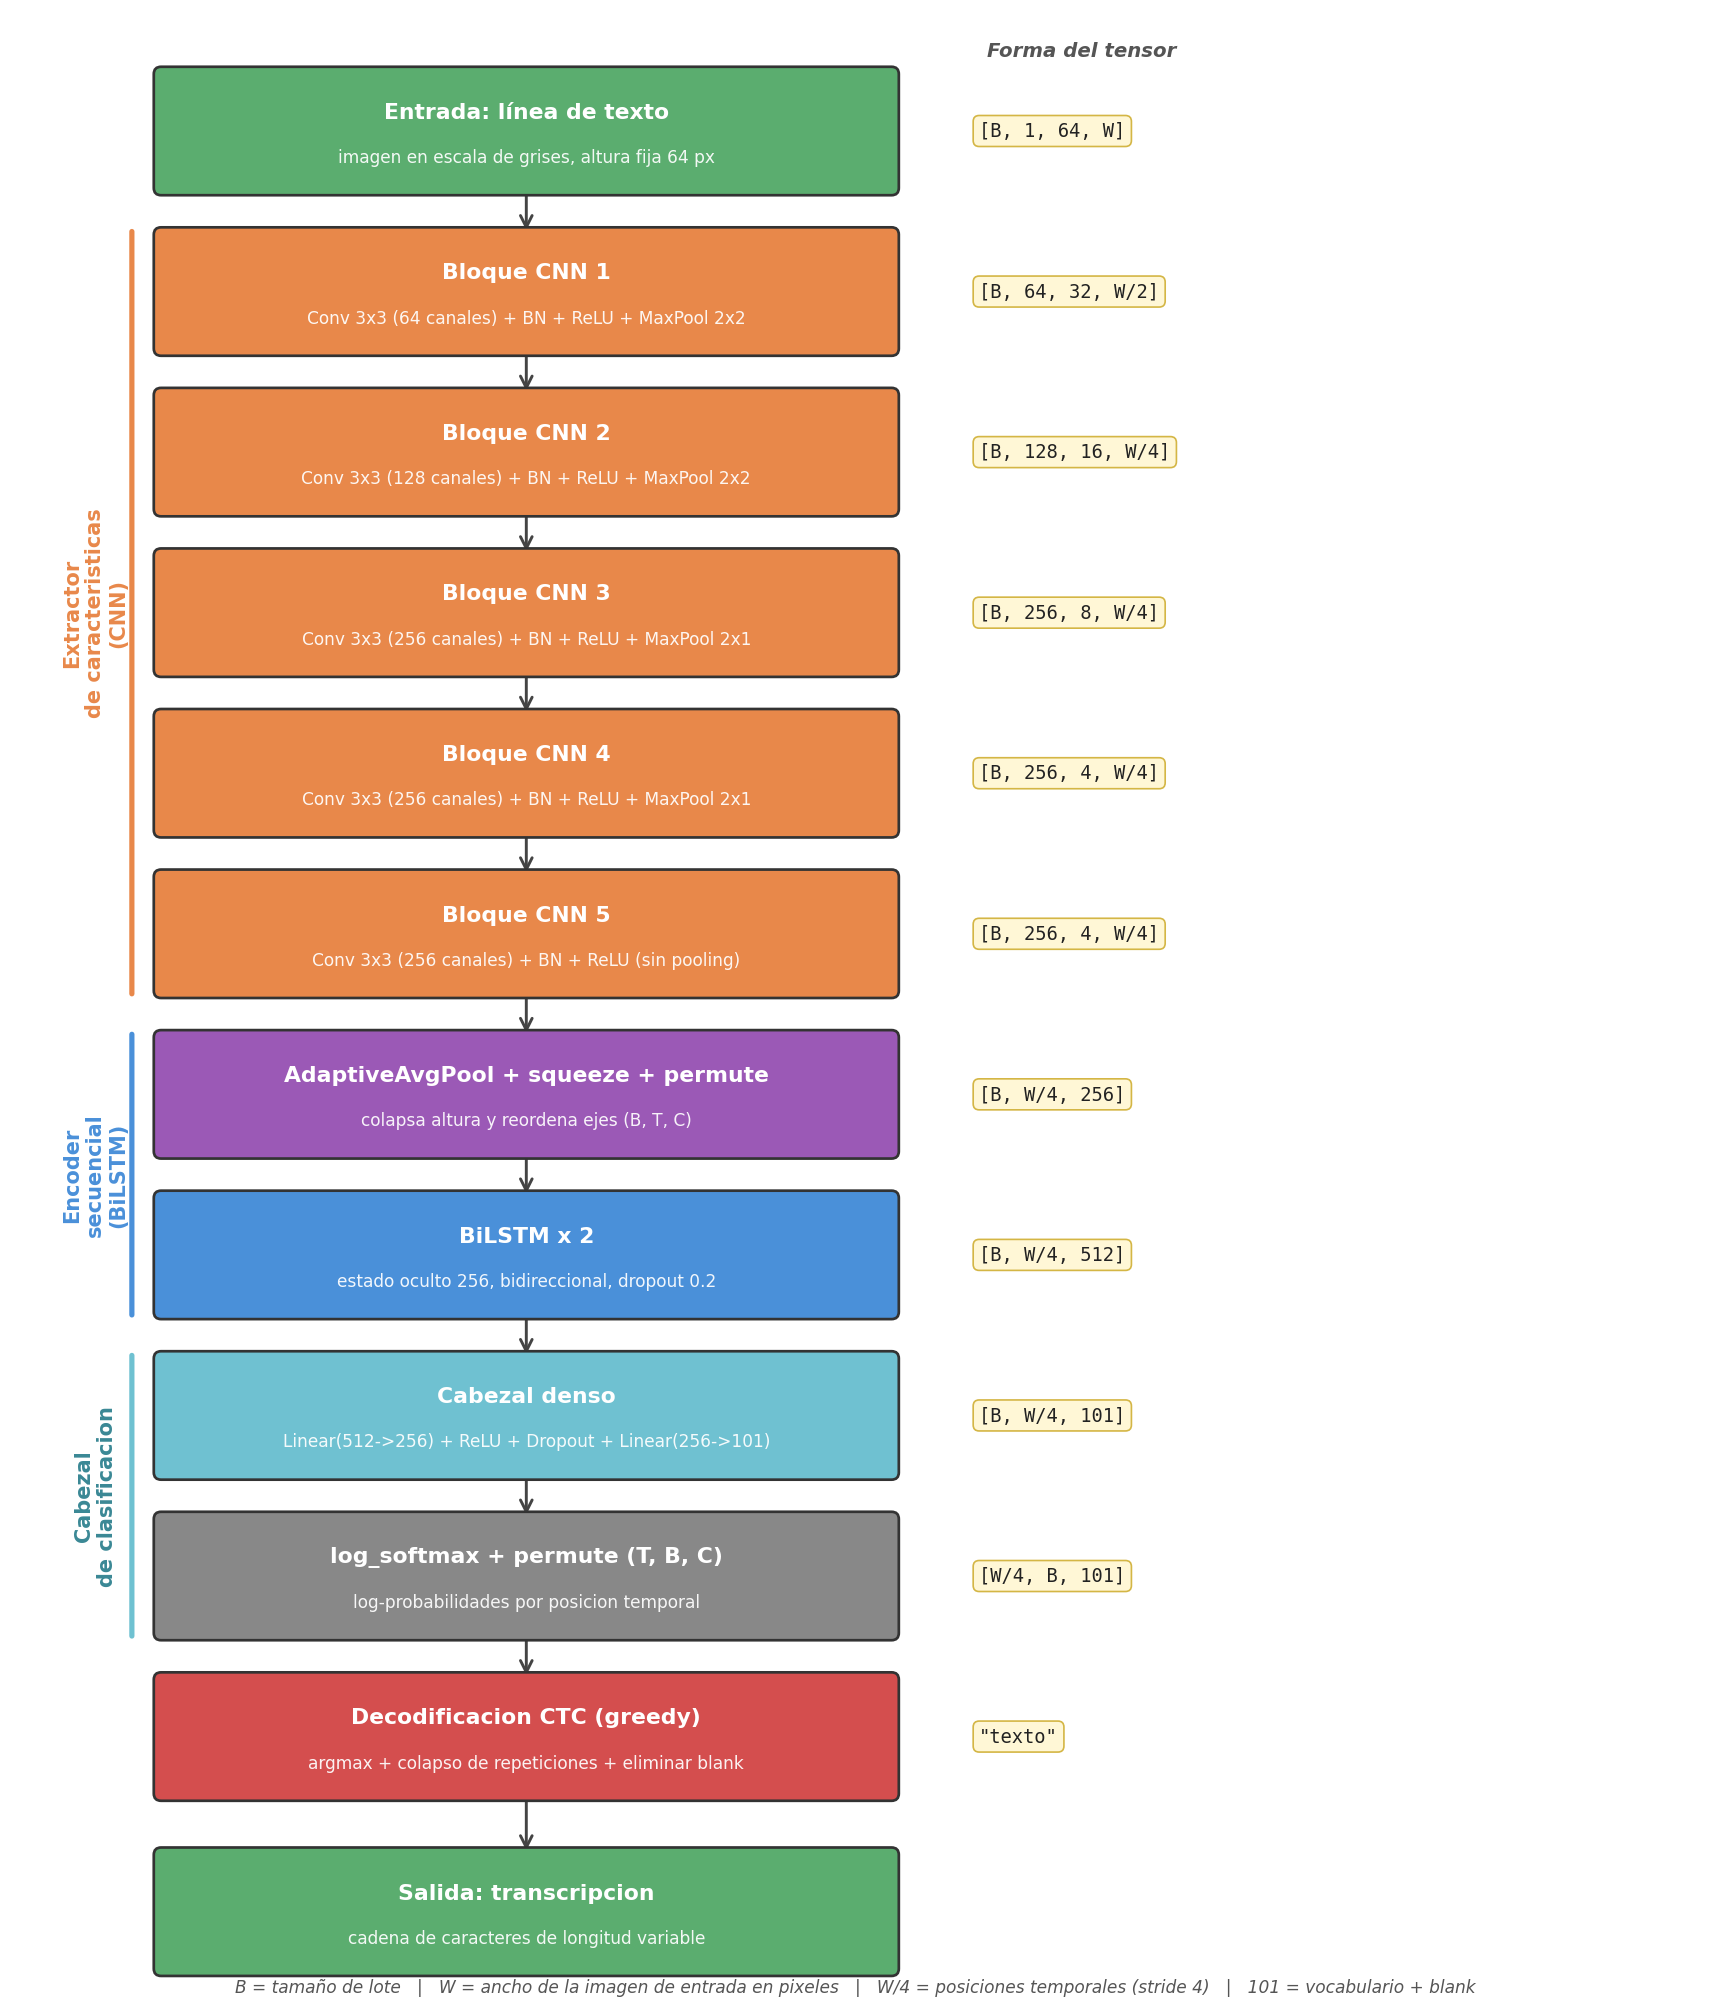
\includegraphics[width=0.92\textwidth]{Graphics/crnn_arquitectura.png}
	\caption{Diagrama del modelo CRNN+CTC para reconocimiento de líneas impresas. Cada caja representa una capa del modelo y la etiqueta amarilla a la derecha indica la forma del tensor a su salida. Las tres etiquetas verticales identifican los tres bloques funcionales: el extractor convolucional (cinco bloques CNN), el codificador secuencial (dos capas BiLSTM apiladas) y el cabezal de clasificación (capas densas seguidas de \textit{log-softmax} y decodificación CTC). El factor de reducción horizontal acumulado de la CNN es cuatro, por lo que el número de posiciones temporales que el modelo produce es la cuarta parte del ancho de la imagen de entrada en píxeles.}
	\label{fig:crnn-arquitectura}
\end{figure}

Las cuatro subsecciones siguientes describen brevemente los componentes y la restricción de longitud que la combinación impone sobre las entradas admisibles.

\subsection{Extractor convolucional}
\label{subsec:cnn-extractor}

El extractor procesa la imagen de la línea y produce una secuencia de vectores de características. Se compone de cinco bloques con \textit{kernel} cuadrado de tres por tres y \textit{padding} unitario, cada uno seguido de normalización por lotes y activación ReLU. Cuatro de los bloques incluyen una operación de \textit{max-pooling}: los dos primeros emplean una ventana cuadrada de dos por dos que reduce ambos ejes a la mitad, y los dos siguientes una ventana asimétrica de dos por uno que reduce solo la altura y preserva la resolución horizontal. La asimetría de los dos últimos \textit{pooling} es el rasgo que permite mantener una secuencia horizontal con resolución suficiente para alimentar al codificador recurrente. La tabla~\ref{tab:bloques-cnn} resume la configuración de los cinco bloques y la forma del tensor a la salida de cada uno.

\begin{table}[!htbp]
	\centering
	\caption{Configuración de los cinco bloques convolucionales del extractor. La columna \emph{Pooling} indica la reducción $(H \times W)$ que la operación aplica.}
	\label{tab:bloques-cnn}
	\footnotesize
	\begin{tabular}{ccccc}
		\toprule
		\textbf{Bloque} & \textbf{Convolución} & \textbf{Pooling} & \textbf{Reducción acumulada} & \textbf{Salida $(C, H, W)$} \\
		\midrule
		1 & Conv $3\times3$, 64 ch  & MaxPool $2\times2$ & $H/2,\ W/2$ & $(64,\ 32,\ W/2)$ \\
		2 & Conv $3\times3$, 128 ch & MaxPool $2\times2$ & $H/4,\ W/4$ & $(128,\ 16,\ W/4)$ \\
		3 & Conv $3\times3$, 256 ch & MaxPool $2\times1$ & $H/8,\ W/4$ & $(256,\ 8,\ W/4)$ \\
		4 & Conv $3\times3$, 256 ch & MaxPool $2\times1$ & $H/16,\ W/4$ & $(256,\ 4,\ W/4)$ \\
		5 & Conv $3\times3$, 256 ch & ---                & $H/16,\ W/4$ & $(256,\ 4,\ W/4)$ \\
		\bottomrule
	\end{tabular}
\end{table}

Una capa de \textit{adaptive-average-pooling} colapsa el eje de altura a uno, una operación de \textit{squeeze} elimina la dimensión unitaria, y una permutación de ejes reordena el resultado como una secuencia indexada por posiciones a lo largo del eje horizontal, con doscientos cincuenta y seis canales por posición. Cada vector codifica las características visuales de una franja vertical de la línea original con un ancho efectivo de cuatro píxeles.

\subsection{Codificador recurrente bidireccional}
\label{subsec:rnn-secuencial}

La secuencia que produce el extractor carece de modelado del contexto entre posiciones vecinas. Una franja vertical aislada es ambigua sin información del contexto adyacente: la franja central de una letra como ``l'' es visualmente indistinguible de la franja central de una letra como ``i'' o ``j'' sin información sobre el resto del trazo. El codificador recurrente aporta el contexto que se necesita para resolver las ambigüedades.

Se emplean dos capas apiladas del tipo \textit{Long Short-Term Memory}~\cite{hochreiter1997lstm}, conocido como LSTM por sus siglas en inglés, en modo bidireccional. La bidireccionalidad consiste en aplicar dos LSTM sobre la misma secuencia, una en sentido directo y otra en sentido inverso, y concatenar las salidas, de modo que cada posición de la secuencia codifica contexto tanto del prefijo como del sufijo. El estado oculto tiene dimensión doscientos cincuenta y seis por dirección, por lo que la salida concatenada en cada posición temporal es un vector de quinientas doce dimensiones.

\subsection{Función de pérdida CTC y \textit{token blank}}
\label{subsec:ctc-loss}

La salida del modelo es una secuencia de distribuciones de probabilidad sobre el vocabulario, indexada por posiciones temporales. La transcripción de referencia es una secuencia de símbolos, indexada por posiciones de la cadena. Las dos secuencias tienen, en general, longitudes distintas y no existe alineamiento explícito entre las posiciones de la primera y las de la segunda. La función de pérdida \textit{Connectionist Temporal Classification}, que el trabajo de Graves et~al.~\cite{graves2006ctc} introdujo originalmente, resuelve el problema sin alineación previa.

La idea central de CTC es introducir un símbolo adicional que la literatura denomina \textit{token blank}, que el modelo puede emitir en cualquier posición temporal sin que aparezca en la transcripción. CTC define la probabilidad de una transcripción como la suma sobre todos los alineamientos posibles entre las posiciones temporales y los símbolos de la transcripción, donde un alineamiento es válido si, tras eliminar las apariciones del \textit{token blank} y colapsar las repeticiones consecutivas del mismo símbolo, produce la transcripción de referencia. El número de alineamientos válidos crece de forma exponencial con la longitud de la secuencia y de la transcripción, por lo que su enumeración explícita es inviable. La pérdida CTC es el logaritmo negativo de la probabilidad agregada de la transcripción, y el algoritmo de \textit{forward-backward}~\cite{graves2006ctc} la calcula en tiempo polinomial mediante programación dinámica, de forma análoga al algoritmo que opera sobre los modelos ocultos de Markov. El algoritmo recorre las posiciones temporales y acumula, para cada par formado por una posición temporal y una posición en la transcripción que intercala \textit{blanks}, la probabilidad agregada de los caminos parciales que llegan a ese estado, lo que permite obtener la probabilidad total sin enumerar caminos individuales.

El \textit{token blank} cumple dos funciones complementarias. La primera es absorber posiciones temporales donde el modelo aún no se compromete con la emisión de un símbolo concreto, condición que se manifiesta como tramos de baja confianza en la salida. La segunda es separar repeticiones legítimas del mismo símbolo: sin \textit{token blank}, una transcripción como ``mejilla'' produciría una sola ``l'' tras el colapso de repeticiones; la presencia del \textit{token blank} entre las dos eles permite preservar la repetición. El vocabulario del sistema contiene los cien símbolos producibles que el capítulo~\ref{chap:corpus} describe, más el \textit{token blank}, que el sistema asigna por convención al índice cien.

\subsection{\textit{Stride} horizontal y restricción de longitud}
\label{subsec:stride-restriccion}

El procesamiento convolucional reduce la dimensión horizontal de la imagen por un factor acumulado de cuatro, según se ve en la tabla~\ref{tab:bloques-cnn}. La consecuencia es que el número de posiciones temporales que el modelo produce es $W/4$, donde $W$ es el ancho de la imagen en píxeles. La función de pérdida CTC requiere que el número de posiciones temporales sea al menos igual a la longitud de la transcripción, ya que cada símbolo debe poder asignarse a al menos una posición temporal en algún alineamiento válido. La condición se traduce en una restricción sobre los pares imagen--transcripción admisibles en entrenamiento:
\begin{equation}
	W \geq 4 \cdot L,
\end{equation}
donde $L$ es la longitud de la transcripción. La generación del \textit{corpus} sintético respeta la restricción, que el capítulo~\ref{chap:corpus} describe, y el análisis exploratorio de la sección~\ref{sec:eda-corpus} confirmó que ninguna imagen del \textit{corpus} de entrenamiento la viola. La sección~\ref{subsec:eda-extendido} reportará la verificación equivalente sobre el \textit{corpus} extendido del \textit{fine-tuning}.

La decisión de adoptar CRNN+CTC en lugar de arquitecturas basadas en transformadores como TrOCR~\cite{li2021trocr} responde a tres factores que el contexto del trabajo impone. El primero es la infraestructura computacional disponible: TrOCR requiere preentrenamiento o adaptación sobre modelos preexistentes que comprenden cientos de millones de parámetros, mientras que CRNN+CTC entrena desde cero sobre el \textit{corpus} sintético propio con 4{,}3 millones de parámetros en una GPU de gama media accesible mediante la plataforma Kaggle. El segundo es la disponibilidad de datos: Laurent y Lauar~\cite{laurent2024spanishtrocr} reportan que la adaptación de TrOCR a texto impreso en español requiere del orden de dos millones de muestras para superar a CRNN+CTC; el \textit{corpus} de este trabajo contiene veinte mil pares imagen--transcripción, dos órdenes de magnitud por debajo del régimen donde la diferencia entre las dos arquitecturas se hace medible. El tercero es el rendimiento observado: el CER del modelo final sobre el conjunto de prueba sintético se sitúa dentro del rango competitivo de los motores OCR de referencia para texto impreso en español según el estado del arte que el capítulo~\ref{chap:estado-arte} describe, lo que indica que la arquitectura CRNN+CTC resulta suficiente para el problema concreto que el trabajo aborda.

% -----------------------------------------------------------------------------
\section{Implementación del modelo}
\label{sec:implementacion-modelo}

La implementación opera en PyTorch~\cite{paszke2019pytorch}. La tabla~\ref{tab:hiperparams-modelo} resume los parámetros estructurales del modelo, que corresponden con la arquitectura que la sección anterior describe.

\begin{table}[!htbp]
	\centering
	\caption{Parámetros estructurales del modelo CRNN+CTC.}
	\label{tab:hiperparams-modelo}
	\begin{tabular}{lc}
		\toprule
		\textbf{Parámetro} & \textbf{Valor} \\
		\midrule
		Altura de entrada                 & 64 píxeles \\
		Tamaño del vocabulario            & 101 (100 símbolos + \textit{blank}) \\
		Bloques convolucionales           & 5 \\
		Canales del extractor             & 64,\ 128,\ 256,\ 256,\ 256 \\
		Tamaño del estado oculto LSTM     & 256 \\
		Capas LSTM apiladas               & 2 \\
		Dirección de la LSTM              & Bidireccional \\
		\textit{Dropout} en cabezal denso & 0,2 \\
		\textit{Stride} horizontal acumulado & 4 \\
		\bottomrule
	\end{tabular}
\end{table}

La inicialización de pesos sigue prácticas habituales para la arquitectura. El sistema inicializa las matrices de entrada de las celdas LSTM~\cite{hochreiter1997lstm} con el esquema de Xavier uniforme~\cite{glorot2010xavier}, que extrae cada peso de una distribución uniforme con varianza calibrada en función del número de entradas y salidas de la capa, de modo que la varianza de las activaciones y de los gradientes se mantenga aproximadamente estable a lo largo de la red y evite tanto la saturación como el desvanecimiento del gradiente. Las matrices recurrentes parten de matrices ortogonales para controlar la propagación de gradientes en secuencias largas. Los sesgos parten de cero, con la única excepción de los sesgos de la puerta de olvido~\cite{gers2000forget}, la compuerta que en cada paso temporal decide qué fracción del estado interno del LSTM mantiene y qué fracción descarta: estos sesgos toman el valor uno, lo que mantiene la puerta abierta al comienzo del entrenamiento y evita que el modelo descarte información antes de aprender a regularla. Las capas densas del cabezal parten también de Xavier uniforme y sesgos a cero.

% -----------------------------------------------------------------------------
\section{Protocolo de entrenamiento}
\label{sec:protocolo-entrenamiento}

El entrenamiento opera sobre el \textit{corpus} sintético que el capítulo~\ref{chap:corpus} describe. El sistema reserva el 10\,\% del \textit{corpus} como conjunto de validación mediante una partición aleatoria con semilla fija que garantiza la reproducibilidad de los experimentos. El protocolo dispone además de un conjunto de prueba independiente que el mismo procedimiento de generación produce con una semilla distinta y que el sistema reserva en exclusiva para la evaluación final del modelo desplegado tras la adaptación por \textit{fine-tuning}, según describe la sección~\ref{sec:test-set}. La sección~\ref{sec:resultados-entrenamiento} complementa la validación con dos procedimientos adicionales para cuantificar la generalización durante el desarrollo, una validación cruzada estratificada por fuente y el experimento de exclusión de una fuente que la subsección~\ref{subsec:cv-lofo} introduce. El procedimiento de generación del \textit{corpus} muestrea cada cadena de texto de forma independiente por fuente tipográfica a partir de las obras de Project Gutenberg, lo que hace despreciable la probabilidad de que un par (cadena, fuente) coincida entre cualesquiera dos de las tres particiones, y elimina la posibilidad de fuga de información entre ellas por solapamiento textual.

La presente sección expone los hiperparámetros, la estrategia de agrupación por ancho que optimiza el uso de memoria de GPU, y las transformaciones de augmentación que el cargador aplica en línea durante el entrenamiento.

\subsection{Hiperparámetros}
\label{subsec:hiperparametros}

La tabla~\ref{tab:hiperparams-entrenamiento} resume los hiperparámetros principales.

\begin{table}[!htbp]
	\centering
	\caption{Hiperparámetros del protocolo de entrenamiento principal.}
	\label{tab:hiperparams-entrenamiento}
	\begin{tabular}{lc}
		\toprule
		\textbf{Hiperparámetro} & \textbf{Valor} \\
		\midrule
		Épocas                         & 30 \\
		Tamaño de lote                 & 32 \\
		Optimizador                    & AdamW \\
		Tasa de aprendizaje máxima     & $3 \times 10^{-4}$ \\
		Decaimiento de pesos           & $10^{-4}$ \\
		Planificador                   & \textit{OneCycleLR} \\
		Recorte de gradiente (norma máx.) & 5,0 \\
		Precisión mixta automática     & Sí \\
		\bottomrule
	\end{tabular}
\end{table}

El optimizador AdamW~\cite{loshchilov2019adamw} emplea la corrección de desacoplamiento del decaimiento de pesos respecto al término de actualización, lo que mejora la generalización respecto al Adam clásico~\cite{kingma2014adam} en presencia de regularización por norma. El planificador \textit{OneCycleLR}~\cite{smith2018onecycle} eleva la tasa de aprendizaje desde un valor pequeño hasta el máximo durante el primer tercio del entrenamiento, y la reduce monótonamente hasta un valor casi nulo durante los dos tercios restantes. La estrategia permite alcanzar valores de tasa de aprendizaje altos en la fase central sin comprometer la estabilidad inicial ni la convergencia final. El recorte de gradiente con norma máxima de cinco protege contra explosiones esporádicas de la magnitud del gradiente en las primeras épocas. La precisión mixta automática emplea representación de coma flotante de dieciséis bits en las operaciones convolucionales y de treinta y dos bits en las acumulaciones críticas, lo que reduce el consumo de memoria y acelera el entrenamiento sin pérdida apreciable de calidad.

\subsection{Agrupación por anchos para optimizar el uso de memoria de GPU}
\label{subsec:bucketing}

Las imágenes del \textit{corpus} presentan anchos variables debido a la diferencia de longitudes de las transcripciones y a la diversidad tipográfica. Una estrategia de carga puramente aleatoria de muestras requiere rellenar cada lote hasta el ancho de la imagen más larga del lote, lo que desperdicia memoria y cómputo en imágenes cortas. Una alternativa que ordene las muestras por ancho elimina el desperdicio pero introduce un sesgo de orden que perjudica la convergencia.

El protocolo emplea un muestreador por agrupamiento, definido en el repositorio del proyecto bajo el nombre \textit{BucketBatchSampler} en el módulo \texttt{Model/dataset.py}
y que combina las dos estrategias. El muestreador ordena las muestras por ancho y las divide en diez grupos contiguos de igual tamaño. Dentro de cada grupo, el muestreador mezcla aleatoriamente las muestras y las reparte en lotes. Mezcla también el orden de los lotes entre grupos. El resultado es un compromiso entre eficiencia del relleno, dado que las imágenes de un mismo lote tienen anchos similares, y aleatoriedad del entrenamiento, ya que cada época presenta los lotes en un orden distinto sin correlación sistemática con el ancho.

\subsection{Augmentación de datos durante el entrenamiento}
\label{subsec:augmentacion-entrenamiento}

Las imágenes del \textit{corpus} sintético, aun con las simulaciones de degradación visual que la sección~\ref{subsec:degradacion} describe, conservan una uniformidad alta respecto a la altura del texto y a la apariencia tipográfica. La augmentación amplía la diversidad efectiva de las muestras mediante transformaciones aleatorias que el cargador aplica en línea a medida que entrega las imágenes al modelo. Cada muestra recibe un conjunto distinto de transformaciones en cada época. El sistema organiza la augmentación en dos etapas independientes que la tabla~\ref{tab:augmentacion} resume.

\begin{table}[!htbp]
	\centering
	\caption{Transformaciones de augmentación que el cargador aplica en línea durante el entrenamiento. El cargador aplica las dos etapas de forma independiente sobre cada muestra; el conjunto de validación recibe las imágenes sin augmentación.}
	\label{tab:augmentacion}
	\begin{tabular}{p{4.2cm}cp{6.0cm}}
		\toprule
		\textbf{Transformación} & \textbf{Probabilidad} & \textbf{Parámetros y propósito} \\
		\midrule
		\multicolumn{3}{l}{\textit{Etapa 1 --- variación de altura previa al redimensionado final}} \\
		\midrule
		Redimensionado aleatorio de altura & $\sim$60\,\% & altura sorteada en $[44, 128]$ px antes del redimensionado final a 64 px; rompe la correspondencia entre forma y tamaño absoluto \\
		\midrule
		\multicolumn{3}{l}{\textit{Etapa 2 --- secuencia de transformaciones sobre la imagen tras el redimensionado}} \\
		\midrule
		Variación del grosor de trazo & $\sim$55\,\%$^\star$ & filtros morfológicos de erosión o dilatación con \textit{kernel} 3$\times$3; cada uno con prob.\ 20\,\% interna \\
		\addlinespace
		Escala horizontal aleatoria & $\sim$55\,\%$^\star$ & factor en $[0{,}70,\ 1{,}40]$; reproduce variaciones de paso tipográfico \\
		\addlinespace
		Distorsión perspectiva & $\sim$55\,\%$^{\star}\!\!\times\!25\,$\% & factor 0,05; simula superficies no planas y escaneos torcidos \\
		\addlinespace
		Variación de brillo y contraste & $\sim$55\,\%$^\star$ & factor 0,25 en ambos; simula iluminación irregular \\
		\addlinespace
		Transformación afín & $\sim$55\,\%$^\star$ & rotación $\pm 3^\circ$, traslación hasta 3\,\% del ancho, \textit{shear} hasta $3^\circ$ \\
		\addlinespace
		\textit{Blur} gaussiano & $\sim$55\,\%$^\star$ & desviación típica en $[0{,}1,\ 1{,}2]$; simula desenfoque óptico \\
		\addlinespace
		Ruido gaussiano (post-normalización) & $\sim$55\,\%$^\star$ & desviación típica hasta 0,05 sobre valores normalizados \\
		\bottomrule
	\end{tabular}
	\vspace{4pt}\\
	\footnotesize $^\star$ El cargador activa o desactiva la etapa 2 globalmente con probabilidad $\sim$55\,\%; cuando la activa, aplica todas las transformaciones de la etapa secuencialmente sobre la misma muestra.
\end{table}

El trabajo elige el conjunto de transformaciones para reproducir la variabilidad que aparece en documentos reales digitalizados sin alterar la legibilidad del texto. La etapa de variación de altura ataca específicamente el riesgo de memorización del tamaño fijo del \textit{corpus} sintético que la sección~\ref{subsec:renderizado} discutió.
ef{subsec:renderizado}.

% -----------------------------------------------------------------------------
\section{Decodificación durante la inferencia}
\label{sec:decodificacion}

Durante la inferencia, el modelo produce la misma secuencia de distribuciones de probabilidad logarítmica que durante el entrenamiento. Un operador de decodificación recorre esas distribuciones y extrae una secuencia de símbolos que constituye la transcripción final. La sección expone las dos estrategias de decodificación que el sistema considera, la comparación empírica entre ambas, y la decisión metodológica de integrar un modelo de lenguaje al componente que opera en producción.

\subsection{Decodificación \textit{greedy}}
\label{subsec:greedy}

La decodificación \textit{greedy} es la estrategia más simple. En cada posición temporal el decoder elige el símbolo con mayor probabilidad. La secuencia que resulta pasa por el posprocesado que el esquema CTC define: el decoder colapsa las repeticiones consecutivas del mismo símbolo y elimina las apariciones del \textit{token blank}. La transcripción resultante es la salida final del sistema. La ventaja es el coste computacional mínimo, con una sola operación de máximo por posición temporal. La desventaja es la incapacidad de explotar dependencias entre posiciones lejanas, ya que el decoder toma cada decisión local sin considerar sus consecuencias sobre las decisiones futuras.

\subsection{Búsqueda en haz}
\label{subsec:beam-search}

La búsqueda en haz, a la que la literatura llama \textit{beam search}~\cite{hannun2014ctcbeam}, mantiene en cada paso un conjunto fijo de las hipótesis parciales con mayor probabilidad acumulada, en lugar de comprometerse con un único símbolo por posición. El conjunto recibe el nombre de haz y su tamaño el de anchura del haz. En cada nueva posición temporal, el decoder extiende cada hipótesis del haz con todos los símbolos del vocabulario, ordena las nuevas hipótesis por probabilidad acumulada y conserva únicamente las mejores. Al final de la secuencia, el decoder devuelve la hipótesis del haz con mayor probabilidad agregada. El coste computacional crece de forma proporcional a la anchura del haz frente al de la decodificación \textit{greedy}.

La búsqueda en haz pura, sin información lingüística externa, no aporta una mejora robusta frente a \textit{greedy} en el esquema CTC. Las hipótesis alternativas que el haz preserva tienen probabilidades acústicas muy próximas a la del argmax, y el decoder carece de criterio para distinguir entre ellas más allá de la propia probabilidad agregada del modelo visual. Cuando el modelo CRNN ya sale con alta confianza carácter a carácter, el haz solo agrega coste computacional. La sección~\ref{subsec:lm-posterior} discute la incorporación de un modelo de lenguaje al esquema, que sí dota al decoder de un criterio adicional para reordenar hipótesis acústicamente compatibles.

\subsection{Comparación empírica sobre validación sintética}
\label{subsec:greedy-vs-beam}

La tabla~\ref{tab:greedy-vs-beam} resume el CER que el protocolo de entrenamiento midió sobre el conjunto de validación con cada una de las dos estrategias. Ambas operan sin información lingüística externa, ya que el modelo de lenguaje quedó fuera del experimento de validación que el protocolo de entrenamiento ejecutó.

\begin{table}[!htbp]
	\centering
	\caption{Comparación de decodificación \textit{greedy} y búsqueda en haz pura sobre el conjunto de validación del modelo final. Ambas estrategias operan sin información lingüística externa.}
	\label{tab:greedy-vs-beam}
	\begin{tabular}{lcl}
		\toprule
		\textbf{Estrategia} & \textbf{CER} & \textbf{Coste por muestra} \\
		\midrule
		Decodificación \textit{greedy}                       & 0,0102 & $\mathcal{O}(T\cdot V)$ \\
		Búsqueda en haz pura (anchura 10, sin LM)            & 0,0172 & $\mathcal{O}(T\cdot V \cdot B)$ \\
		\bottomrule
	\end{tabular}
\end{table}

El resultado tiene una causa identificable. La validación sintética consta de líneas tipográficamente limpias, sin degradaciones de escaneo ni ruidos de captura. El modelo CRNN sale carácter a carácter con alta confianza: el segundo y el tercer candidato por probabilidad están lejos del primero, y la distribución de salida sobre el vocabulario es marcadamente puntiaguda. En este régimen el argmax acierta casi siempre, y la búsqueda en haz mantiene hipótesis alternativas que apenas se diferencian del argmax. Sin un criterio externo de reordenamiento, el haz no encuentra señal sobre la que actuar y a veces termina favoreciendo hipótesis ligeramente peores, lo que explica que el CER del beam puro supere al del \textit{greedy}. El protocolo de entrenamiento adopta la decodificación \textit{greedy} para la evaluación que la sección~\ref{sec:resultados-entrenamiento} reporta.

\subsection{Integración posterior de un modelo de lenguaje en producción}
\label{subsec:lm-posterior}

Tras el cierre del protocolo de entrenamiento, el desarrollo del sistema en producción incorpora un modelo de lenguaje a la inferencia. La motivación reside en la diferencia entre la naturaleza de la validación sintética y la naturaleza de los documentos reales que el sistema procesa cuando opera en su contexto de uso.

El modelo de lenguaje opera como un \textit{n-gram} de orden cinco a nivel de carácter, preentrenado sobre corpus de español de uso general, que la herramienta KenLM~\cite{heafield2011kenlm} carga y consulta durante la inferencia. La integración consiste en una variante de la búsqueda en haz que, además de la probabilidad acústica del modelo CRNN, pondera cada hipótesis con la probabilidad que el modelo de lenguaje asigna a la secuencia de caracteres correspondiente. La combinación de las dos fuentes de información sigue una combinación lineal de logaritmos con peso $\alpha = 0{,}4$ para el modelo de lenguaje, anchura de haz igual a diez y un término de normalización por longitud con exponente 0,65 que compensa la tendencia del decoder a favorecer hipótesis cortas.

Los documentos reales presentan dos propiedades que la validación sintética no replica con la misma fuerza. La primera es la mayor incertidumbre del modelo visual carácter a carácter. Las degradaciones del escaneado, las tipografías inusuales y las variaciones de tamaño y de contraste producen distribuciones de salida menos puntiagudas que sobre la validación sintética. El segundo y el tercer candidato por probabilidad se acercan al primero, lo que abre un margen donde la búsqueda en haz mantiene varias hipótesis apreciablemente distintas en lugar de comprometerse en cada paso con la más probable. La segunda propiedad es la regularidad morfológica y ortográfica del español formal. El modelo de lenguaje 5-gram de caracteres aprende patrones recurrentes a nivel local: sufijos productivos como ``-ción'', ``-mente'' o ``-dad'', terminaciones verbales como ``-aba'', ``-aron'' o ``-ería'', las reglas ortográficas obligatorias que el español aplica a las combinaciones ``qu'' y ``gu'', donde la vocal siguiente solo puede ser ``e'' o ``i'', y los patrones de tildación. Cuando la búsqueda en haz mantiene varias hipótesis acústicamente compatibles, el modelo de lenguaje reordena las hipótesis en favor de la que forma una secuencia morfológicamente plausible del idioma.

La combinación de las dos propiedades explica la diferencia entre los dos escenarios. En la validación sintética el modelo visual ya está casi seguro carácter a carácter, y el reordenamiento por el modelo de lenguaje apenas cambia las hipótesis. En documentos reales la incertidumbre acústica deja espacio para que la información lingüística marque la diferencia. La decisión de integrar el modelo de lenguaje en producción descansa sobre este principio y sobre la observación del comportamiento del sistema en su entorno de despliegue.

La validación cuantitativa de la mejora sobre el conjunto de prueba sintético no es metodológicamente correcta. El \textit{corpus} de entrenamiento, según describe el capítulo~\ref{chap:corpus}, surge de un procedimiento de muestreo por déficit que equilibra las frecuencias de caracteres del español y que rompe deliberadamente la cohesión léxica del idioma para amplificar las clases minoritarias. Las cadenas resultantes constan de secuencias de tokens válidos cosidos artificialmente, sin las transiciones que caracterizan al español natural. Un modelo de lenguaje que el preentrenamiento ajustó sobre español fluido no encuentra patrones que aportar sobre cadenas que no son fluidas, y la medición sobre material sintético subestimaría sistemáticamente el aporte del LM al ofrecerle un terreno donde la información lingüística que codifica no tiene aplicación. El conjunto de prueba que la sección~\ref{sec:test-set} describe hereda esta propiedad y la misma razón lo excluye como banco de evaluación del componente lingüístico.

El trabajo evalúa el aporte del LM sobre líneas reales obtenidas de varios documentos, en una inspección cualitativa cuyo objetivo es observar el tipo de correcciones que el LM produce sobre material genuino. La figura~\ref{fig:kenlm-cualitativo} presenta tres ejemplos representativos en los que la decodificación \textit{beam}+LM difiere de la \textit{greedy}.

\begin{figure}[!htbp]
\centering

\begin{minipage}{0.97\linewidth}
\centering
\fbox{
\includegraphics[width=0.95\linewidth]{Graphics/kenlm_ej1_anos.jpg}}
\par\vspace{0.4em}
{\scriptsize
\begin{tabular}{@{}rl@{}}
\textbf{Imagen}   & \textit{aminación de esta zona con bacterias procedentes del ano.} \\
\textbf{Greedy}   & \texttt{aminación de esta zona con bacterias procedentes del \textcolor{red!70!black}{anos}} \\
\textbf{Beam+LM} & \texttt{aminación de esta zona con bacterias procedentes del \textcolor{green!50!black}{ano}} \\
\end{tabular}}
\end{minipage}

\vspace{1em}

\begin{minipage}{0.97\linewidth}
\centering
\fbox{
\includegraphics[width=0.95\linewidth]{Graphics/kenlm_ej2_puntuacion.jpg}}
\par\vspace{0.4em}
{\scriptsize
\begin{tabular}{@{}rl@{}}
\textbf{Imagen}   & \textit{capital de la insurrección? Al cono-} \\
\textbf{Greedy}   & \texttt{capital de la insurrección \textcolor{red!70!black}{?} \textcolor{red!70!black}{A'} cono-} \\
\textbf{Beam+LM} & \texttt{capital de la insurrección\textcolor{green!50!black}{?} \textcolor{green!50!black}{A} cono-} \\
\end{tabular}}
\end{minipage}

\vspace{1em}

\begin{minipage}{0.97\linewidth}
\centering
\fbox{
\includegraphics[width=0.95\linewidth]{Graphics/kenlm_ej3_ua.jpg}}
\par\vspace{0.4em}
{\scriptsize
\begin{tabular}{@{}rl@{}}
\textbf{Imagen}   & \textit{Cuba que la insurrección se había extendido por gran parte de Oriente,} \\
\textbf{Greedy}   & \texttt{Cuba que \textcolor{red!70!black}{Úa} insurrección se había extendido por gran parte de Oriente.} \\
\textbf{Beam+LM} & \texttt{Cuba que \textcolor{green!50!black}{la} insurrección se había extendido por gran parte de Oriente} \\
\end{tabular}}
\end{minipage}

\caption[Comparación cualitativa entre \textit{greedy} y \textit{beam}+LM sobre líneas reales.]{Comparación cualitativa entre la decodificación \textit{greedy} y la decodificación con búsqueda en haz más modelo de lenguaje (\textit{beam}+LM) sobre tres líneas reales del archivo del centro Juan Marinello. En cada panel: la imagen original (arriba), la transcripción visualmente correcta (Imagen), la salida del decodificador voraz (Greedy) y la salida del decodificador con LM (Beam+LM). En rojo, los errores del decodificador voraz; en verde, las correcciones del LM.}
\label{fig:kenlm-cualitativo}
\end{figure}

Los tres ejemplos ilustran tres mecanismos distintos del LM. En el primero, el decodificador voraz añade una \emph{s} terminal a la palabra ``ano'', y produce una secuencia (``anos'') que el modelo visual considera ligeramente más probable carácter a carácter pero que el contexto sintáctico inmediato no admite; el LM, al ponderar el final de la cadena con su probabilidad lingüística, prefiere la hipótesis sin la \emph{s} espuria. En el segundo, el decodificador voraz inserta un espacio antes del signo de interrogación de cierre y un apóstrofo tras una mayúscula aislada, secuencias que el español no contempla en esa posición; el LM elimina ambos artefactos. En el tercero, el decodificador voraz produce ``Úa'' como inicio de palabra, secuencia que no aparece en el léxico del español; el LM la sustituye por ``la'', la única alternativa acústicamente próxima que sí es una palabra del idioma. Los tres mecanismos --corrección de sufijo léxico, limpieza de puntuación ortográfica, sustitución por palabra real-- responden a regularidades del español formal que el modelo de lenguaje codificó durante su preentrenamiento sobre \textit{corpus} de uso general.

La evidencia cualitativa confirma el principio teórico que justifica la integración del LM en producción y aporta una caracterización del tipo de mejoras que el componente introduce. La cuantificación rigurosa de la magnitud de la mejora sobre documentos reales exige un \textit{benchmark} con transcripciones de referencia validadas humanamente y queda como línea de trabajo futuro que el capítulo de recomendaciones recoge.

% -----------------------------------------------------------------------------
\section{Protocolo de evaluación estadística}
\label{sec:evaluacion-estadistica}

La evaluación del modelo durante el desarrollo opera sobre el conjunto de validación, sin augmentación, mediante las métricas CER, WER y exactitud por línea~\cite{jurafsky2024slp} que la sección~\ref{sec:metricas} del capítulo~\ref{chap:estado-arte} define. La evaluación final del modelo desplegado opera, además, sobre el conjunto de prueba independiente que la sección~\ref{sec:test-set} describe. Un protocolo estadístico complementa las métricas puntuales y cuantifica la incertidumbre de las estimaciones, lo que permite comparaciones rigurosas entre configuraciones. La presente sección describe los tres componentes del protocolo estadístico: el cálculo de intervalos de confianza por remuestreo, las pruebas no paramétricas para comparación entre configuraciones, y los experimentos de validación cruzada y de fuente que queda fuera del entrenamiento.

\subsection{Intervalos de confianza por \textit{bootstrap}}
\label{subsec:bootstrap}

El método \textit{bootstrap}~\cite{efron1979bootstrap} construye una distribución empírica del estimador de interés mediante remuestreo con reemplazo del conjunto de evaluación. El protocolo genera diez mil remuestreos del conjunto de validación, calcula la métrica sobre cada remuestreo y construye el intervalo de confianza al 95\,\% como el rango entre los percentiles 2,5 y 97,5 de la distribución que resulta.

Dos consideraciones justifican la elección del \textit{bootstrap}~\cite{efron1979bootstrap} por encima de fórmulas analíticas. La primera es la naturaleza de las métricas: el CER es una proporción agregada sobre la totalidad de los caracteres del conjunto, no una media simple de mediciones independientes, lo que invalida la aplicación directa de las fórmulas clásicas para intervalos de confianza de medias. La segunda es la marcada asimetría de la distribución del error por muestra, que la sección~\ref{subsec:tests} caracteriza con la prueba de Shapiro-Wilk y que invalida cualquier procedimiento paramétrico que descanse sobre supuestos gaussianos. El \textit{bootstrap} no requiere supuestos sobre la forma de la distribución y permite construir intervalos de confianza válidos sobre cualquier estimador.

\subsection{Pruebas no paramétricas para comparación entre configuraciones}
\label{subsec:tests}

La comparación entre configuraciones del modelo requiere pruebas estadísticas que no asuman normalidad de la distribución del error. La elección entre el conjunto de pruebas paramétricas, cuya aplicabilidad depende de que los datos sigan una distribución gaussiana, y el conjunto de pruebas no paramétricas, que opera con supuestos más débiles, descansa sobre una prueba previa de normalidad que opera sobre la distribución del CER por muestra. El protocolo emplea la prueba de Shapiro-Wilk~\cite{shapiro1965normality}, que la literatura estadística considera uno de los tests más potentes para detectar desviaciones de la normalidad en muestras de tamaño moderado y grande. La hipótesis nula del test es que la muestra procede de una distribución normal; el rechazo de la hipótesis nula indica que cualquier procedimiento paramétrico que asuma normalidad pierde su validez teórica.

El protocolo aplicó el test al CER por muestra del modelo final sobre el conjunto de validación, con $n = 1\,999$ muestras. El resultado fue el estadístico $W = 0{,}3095$ y un valor de probabilidad $p = 1{,}42 \times 10^{-65}$. El rechazo de la hipótesis de normalidad es contundente y deja a las pruebas no paramétricas como única opción metodológicamente correcta. El resultado concuerda con la naturaleza del error: la distribución del CER por muestra es marcadamente asimétrica y multimodal, con una masa concentrada en cero (líneas que el modelo transcribe sin error) y una cola larga hacia valores altos (líneas donde el modelo acumula errores). Ninguna transformación habitual aproxima esta distribución a una gaussiana.

El protocolo emplea las tres pruebas no paramétricas que la tabla~\ref{tab:tests-estadisticos} resume, cada una adecuada a un tipo distinto de comparación.

\begin{table}[!htbp]
	\centering
	\caption{Pruebas estadísticas que el protocolo emplea. Todas son no paramétricas y no asumen normalidad de los errores.}
	\label{tab:tests-estadisticos}
	\begin{tabular}{p{3.0cm}p{4.5cm}p{6.0cm}}
		\toprule
		\textbf{Prueba} & \textbf{Métrica que compara} & \textbf{Aplicación en el protocolo} \\
		\midrule
		Wilcoxon de los rangos con signo &
		Diferencias del CER por muestra entre dos configuraciones &
		Comparar decodificaciones \textit{greedy} vs.\ \textit{beam search} sobre las mismas muestras (datos pareados) \\
		\addlinespace
		McNemar &
		Tabla $2\times 2$ de líneas correctas o incorrectas en cada configuración &
		Comparar la exactitud por línea entre dos configuraciones; con corrección de continuidad de Edwards si hay menos de 25 discordancias \\
		\addlinespace
		Kruskal-Wallis &
		Distribución del CER entre múltiples grupos &
		Comparar el error medio del modelo entre las distintas fuentes tipográficas \\
		\bottomrule
	\end{tabular}
\end{table}

\subsection{Validación cruzada y experimento \textit{Leave-One-Font-Out}}
\label{subsec:cv-lofo}

El conjunto de validación, que el protocolo separa aleatoriamente del \textit{corpus}, sigue la misma distribución que el de entrenamiento. Las métricas sobre validación, aun siendo informativas, no estiman la capacidad del modelo de generalizar a fuentes tipográficas o registros visuales que el entrenamiento no observó. Para evaluar la generalización, el protocolo incluye dos experimentos complementarios.

El primero es la validación cruzada estratificada~\cite{kohavi1995cv} por fuente tipográfica, que divide el \textit{corpus} en cinco particiones que conservan la proporción de imágenes de cada fuente, y entrena el modelo cinco veces, cada una con una partición distinta como conjunto de validación. El experimento estima la variabilidad de las métricas frente a la partición aleatoria del \textit{corpus}.

El segundo es el experimento \textit{Leave-One-Font-Out}~\cite{etter2019synthrecipe}, que la literatura abrevia LOFO, sobre el cual el protocolo ejecuta nueve entrenamientos sucesivos. Cada uno excluye una fuente tipográfica del entrenamiento y evalúa sobre la fuente que quedó fuera. El experimento cuantifica la capacidad de generalización del modelo a fuentes que no vio durante el entrenamiento. La diferencia entre el CER promedio sobre las fuentes que quedaron fuera y el CER sobre el conjunto de validación habitual mide la degradación que cabe esperar cuando el sistema encuentra una tipografía nueva en producción.

% -----------------------------------------------------------------------------
\section{Resultados experimentales del entrenamiento principal}
\label{sec:resultados-entrenamiento}

El protocolo entrena el modelo durante treinta épocas sobre las nueve fuentes tipográficas del \textit{corpus}. Todas las métricas que esta sección reporta corresponden a la evaluación con decodificación \textit{greedy} sobre el conjunto de validación sintética, que es el decoder que el protocolo de entrenamiento adoptó por las razones que la sección~\ref{subsec:greedy-vs-beam} expone. El sistema en producción emplea el decoder con modelo de lenguaje que la sección~\ref{subsec:lm-posterior} describe; las métricas del entrenamiento sirven como indicador de seguimiento del modelo visual durante el entrenamiento. La figura~\ref{fig:curvas-entrenamiento} muestra la trayectoria de las tres métricas de error sobre el conjunto de validación a lo largo de las treinta épocas.

\begin{figure}[!htbp]
	\centering
	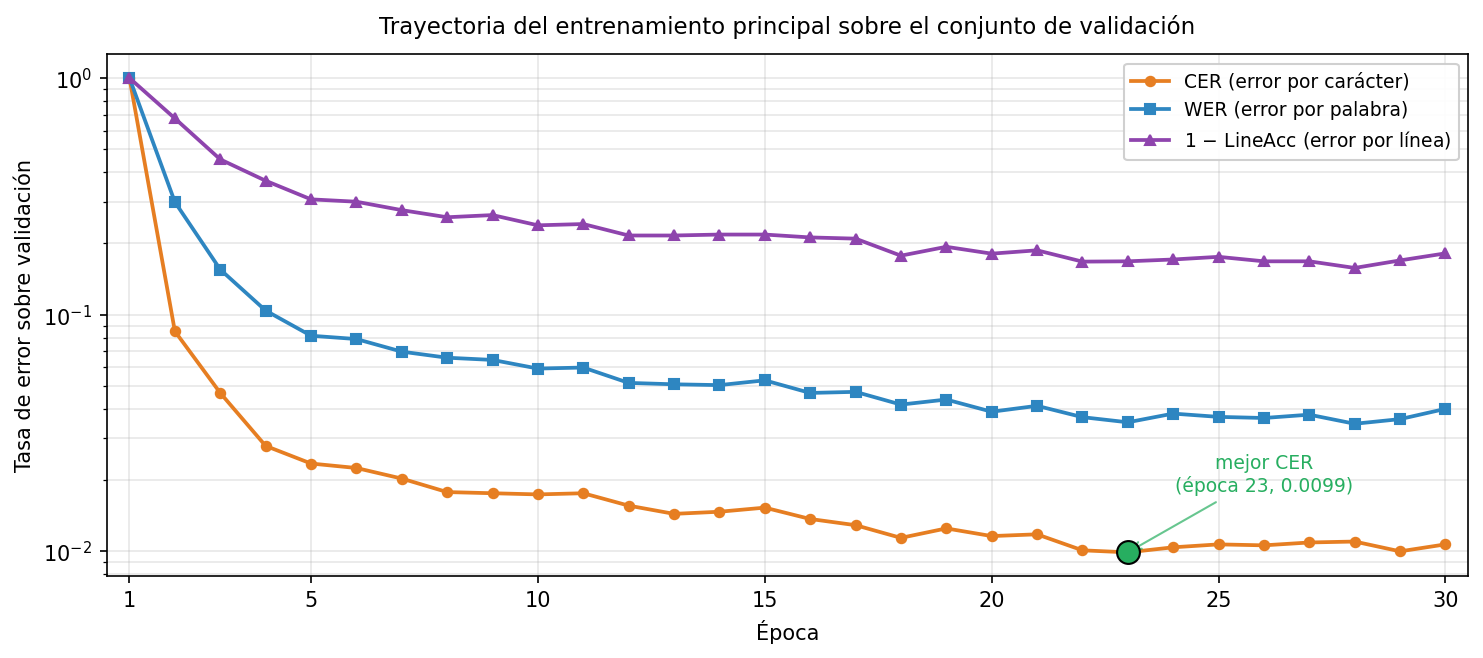
\includegraphics[width=\textwidth]{Graphics/curvas_entrenamiento.png}
	\caption{Trayectoria de las tres métricas de error sobre el conjunto de validación sintética con decodificación \textit{greedy}, a lo largo de las treinta épocas del entrenamiento principal: CER (error por carácter, en naranja), WER (error por palabra, en azul) y la tasa de error por línea, que resulta de restar la exactitud por línea a uno (en morado). Los tres ejes son escalas logarítmicas para que la caída inicial de tres órdenes de magnitud y el régimen estacionario posterior sean ambos legibles. El marcador verde señala la época veintitrés, donde el CER alcanza su valor mínimo de 0,0099 y de la cual procede el \textit{checkpoint} que producción emplea. La trayectoria conjunta de las tres métricas en el mismo eje permite contrastar la velocidad relativa de mejora de cada nivel de granularidad: el error por carácter cae más rápido y se estabiliza antes que el error por palabra, y este a su vez antes que el error por línea, lo que refleja la naturaleza multiplicativa de los errores a lo largo de una secuencia.}
	\label{fig:curvas-entrenamiento}
\end{figure}

La figura~\ref{fig:curvas-loss-lr} complementa la información anterior con la trayectoria de la pérdida CTC y del programador de tasa de aprendizaje a lo largo del entrenamiento. La pérdida de validación y la media por época de la pérdida de entrenamiento siguen trayectorias paralelas, con una separación que se mantiene por debajo de 0,02 unidades a lo largo del entrenamiento, lo que indica que el modelo no presenta sobreajuste medible al final de las treinta épocas. El programador \textit{OneCycleLR} eleva la tasa de aprendizaje desde un valor cercano a $10^{-5}$ en los primeros lotes hasta el máximo de $3 \times 10^{-4}$ en torno a la cuarta época, y la reduce de forma monótona hasta valores próximos a $10^{-8}$ en las últimas épocas para favorecer la convergencia del modelo.

\begin{figure}[!htbp]
	\centering
	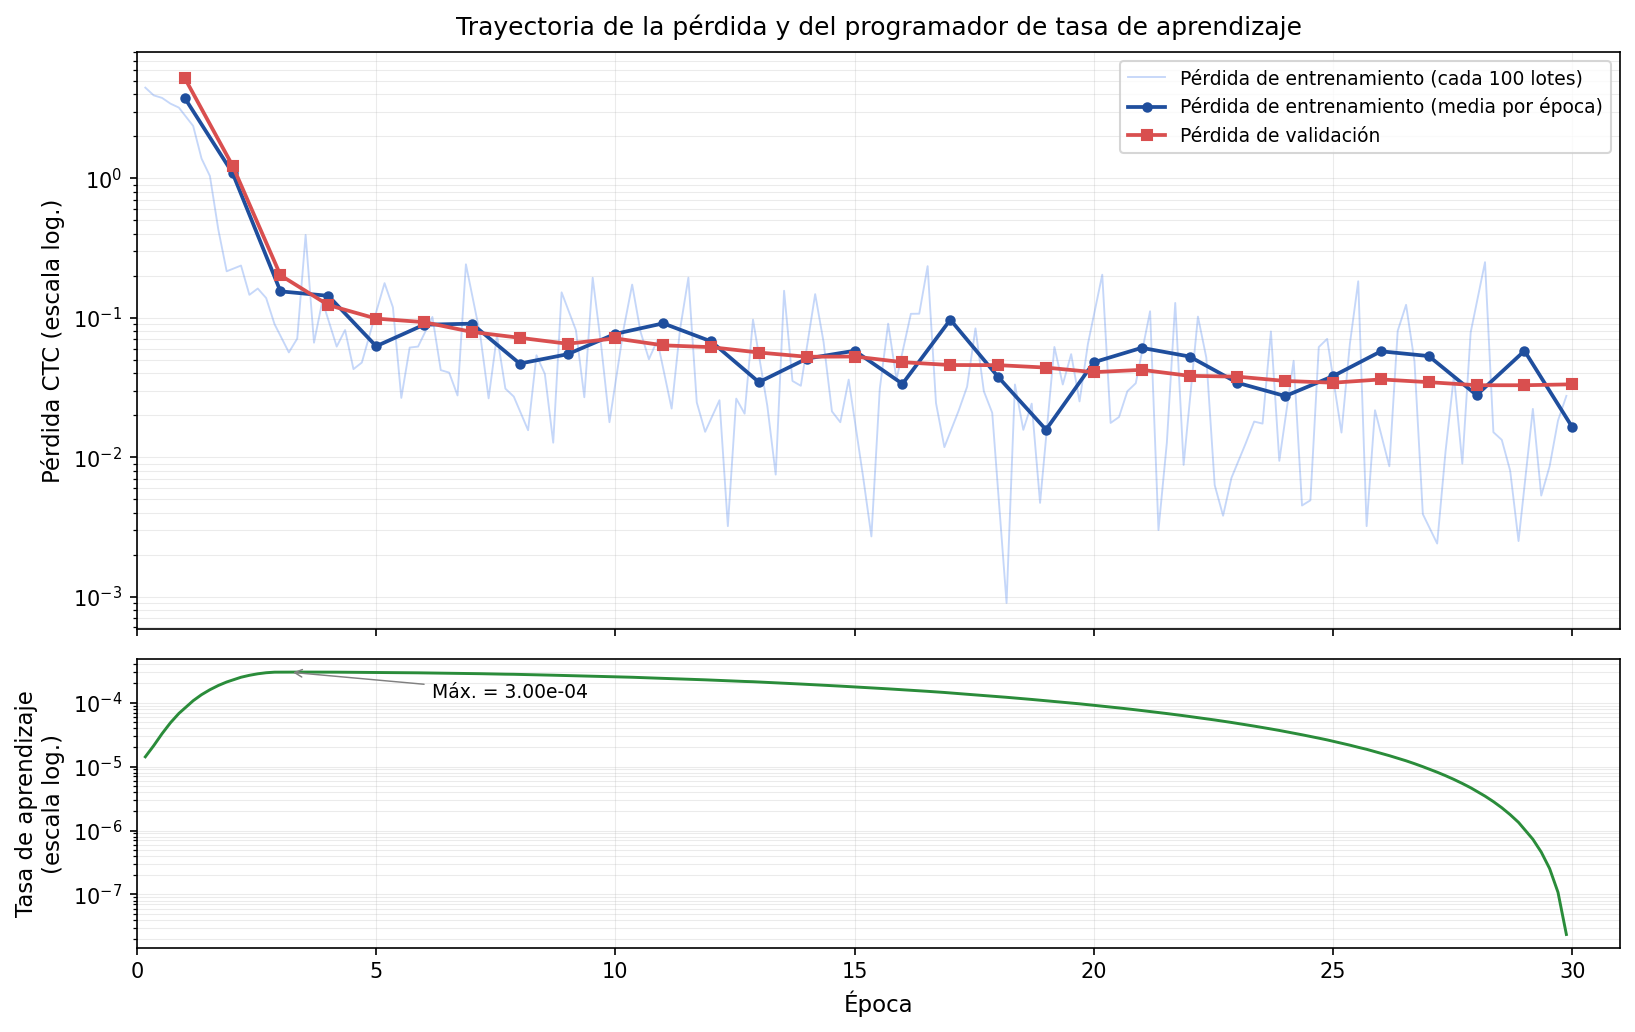
\includegraphics[width=\textwidth]{Graphics/curvas_loss_lr.png}
	\caption{Trayectoria de la pérdida CTC y del programador de tasa de aprendizaje a lo largo de las treinta épocas del entrenamiento principal. El panel superior reporta la pérdida de validación (línea roja con marcadores cuadrados), la media por época de la pérdida de entrenamiento (línea azul oscura con marcadores circulares) y la pérdida de entrenamiento por lote, muestreada cada cien lotes y representada en transparencia para no ocultar las medias. El panel inferior reporta la tasa de aprendizaje que el programador \textit{OneCycleLR} aplica a lo largo del entrenamiento. Los dos ejes verticales emplean escala logarítmica.}
	\label{fig:curvas-loss-lr}
\end{figure}

La pérdida cae más de dos órdenes de magnitud durante las primeras cinco épocas, y el modelo alcanza un CER inferior a 0,03 en la quinta época. A partir de la décima época la mejora se ralentiza y el CER oscila entre 0,01 y 0,02 hasta el final del entrenamiento. La tabla~\ref{tab:resultados-principal} resume las métricas que el modelo final alcanza con decodificación \textit{greedy} sobre el conjunto de validación, con intervalos de confianza al 95\,\% que el procedimiento \textit{bootstrap} produce.

\begin{table}[!htbp]
	\centering
	\caption{Resultados del entrenamiento principal sobre el conjunto de validación. La columna \emph{Std} reporta la desviación típica de la métrica por muestra; el procedimiento \textit{bootstrap} con diez mil remuestreos produce los intervalos de confianza al 95\,\%. La marcada asimetría de las distribuciones por muestra explica que la \emph{Std} alcance un orden de magnitud comparable o superior al de la media, ya que el modelo transcribe la mayoría de las líneas sin errores y un pequeño grupo concentra todos los errores. Esta asimetría justifica el recurso a tests no paramétricos.}
	\label{tab:resultados-principal}
	\begin{tabular}{lccc}
		\toprule
		\textbf{Métrica} & \textbf{Media} & \textbf{Std} & \textbf{IC 95\,\%} \\
		\midrule
		CER             & 0,0106 & 0,0374 & $[0{,}0090,\ 0{,}0122]$ \\
		WER             & 0,0374 & 0,1012 & $[0{,}0331,\ 0{,}0419]$ \\
		Exactitud por línea & 0,8269 & 0,3783 & $[0{,}8099,\ 0{,}8434]$ \\
		\bottomrule
	\end{tabular}
\end{table}

La tasa de error de carácter inferior al 1,1\,\% sitúa el sistema en un rango competitivo con los motores OCR para texto impreso en español, según discutió la sección~\ref{sec:estado-arte} del capítulo~\ref{chap:estado-arte}. La exactitud por línea próxima al 83\,\% indica que cuatro de cada cinco líneas reciben transcripción sin ningún error. La prueba binomial exacta sobre la exactitud por línea contrasta la hipótesis nula de un clasificador aleatorio con probabilidad 0,5 por línea frente a la alternativa de probabilidad superior, y la rechaza con un valor de probabilidad inferior a $10^{-200}$, lo que confirma la superioridad estadística del modelo sobre cualquier clasificador trivial.

El análisis por fuente tipográfica se resume en la tabla~\ref{tab:cer-por-fuente-principal}. La prueba de Kruskal-Wallis~\cite{kruskal1952ranks} sobre las nueve fuentes no rechaza la hipótesis de igualdad de distribuciones del CER entre fuentes, con $H = 11{,}93$ y valor de probabilidad $p = 0{,}154$. El resultado indica que el modelo no presenta un sesgo sistemático a favor de ninguna familia tipográfica del \textit{corpus} original.

\begin{table}[!htbp]
	\centering
	\caption{CER por fuente tipográfica sobre el conjunto de validación del entrenamiento principal. La columna \emph{Std} reporta la desviación típica del CER por muestra dentro de la fuente. Las nueve fuentes se ordenan alfabéticamente.}
	\label{tab:cer-por-fuente-principal}
	\begin{tabular}{lccc}
		\toprule
		\textbf{Fuente} & \textbf{CER} & \textbf{Std} & \textbf{IC 95\,\%} \\
		\midrule
		CourierPrime      & 0,0093 & 0,0405 & $[0{,}0047,\ 0{,}0152]$ \\
		CrimsonPro        & 0,0118 & 0,0375 & $[0{,}0071,\ 0{,}0171]$ \\
		CutiveMono        & 0,0083 & 0,0302 & $[0{,}0049,\ 0{,}0126]$ \\
		EBGaramond        & 0,0139 & 0,0424 & $[0{,}0088,\ 0{,}0199]$ \\
		Inconsolata       & 0,0101 & 0,0346 & $[0{,}0058,\ 0{,}0153]$ \\
		JetBrainsMono     & 0,0102 & 0,0401 & $[0{,}0057,\ 0{,}0157]$ \\
		LibreBaskerville  & 0,0119 & 0,0343 & $[0{,}0078,\ 0{,}0164]$ \\
		RobotoMono        & 0,0123 & 0,0460 & $[0{,}0072,\ 0{,}0187]$ \\
		SpecialElite      & 0,0076 & 0,0256 & $[0{,}0045,\ 0{,}0114]$ \\
		\bottomrule
	\end{tabular}
\end{table}

La validación cruzada estratificada por fuente que la subsección~\ref{subsec:cv-lofo} introduce permite cuantificar la sensibilidad del rendimiento frente a la partición aleatoria del \textit{corpus}. El protocolo divide las 19\,998 imágenes en cinco particiones que conservan la proporción de imágenes de cada fuente. Cada repetición entrena el modelo desde cero con cuatro particiones como entrenamiento y la quinta como validación, durante doce épocas. El número reducido de épocas respecto al entrenamiento principal mantiene el coste computacional total en un orden manejable y resulta suficiente para estimar la variabilidad de las métricas, que es el objetivo del experimento, sin necesidad de alcanzar el mejor modelo posible en cada repetición. La figura~\ref{fig:cv-5fold} presenta las trayectorias del CER por época sobre la partición de validación de cada repetición, junto con el CER final por partición.

\begin{figure}[!htbp]
	\centering
	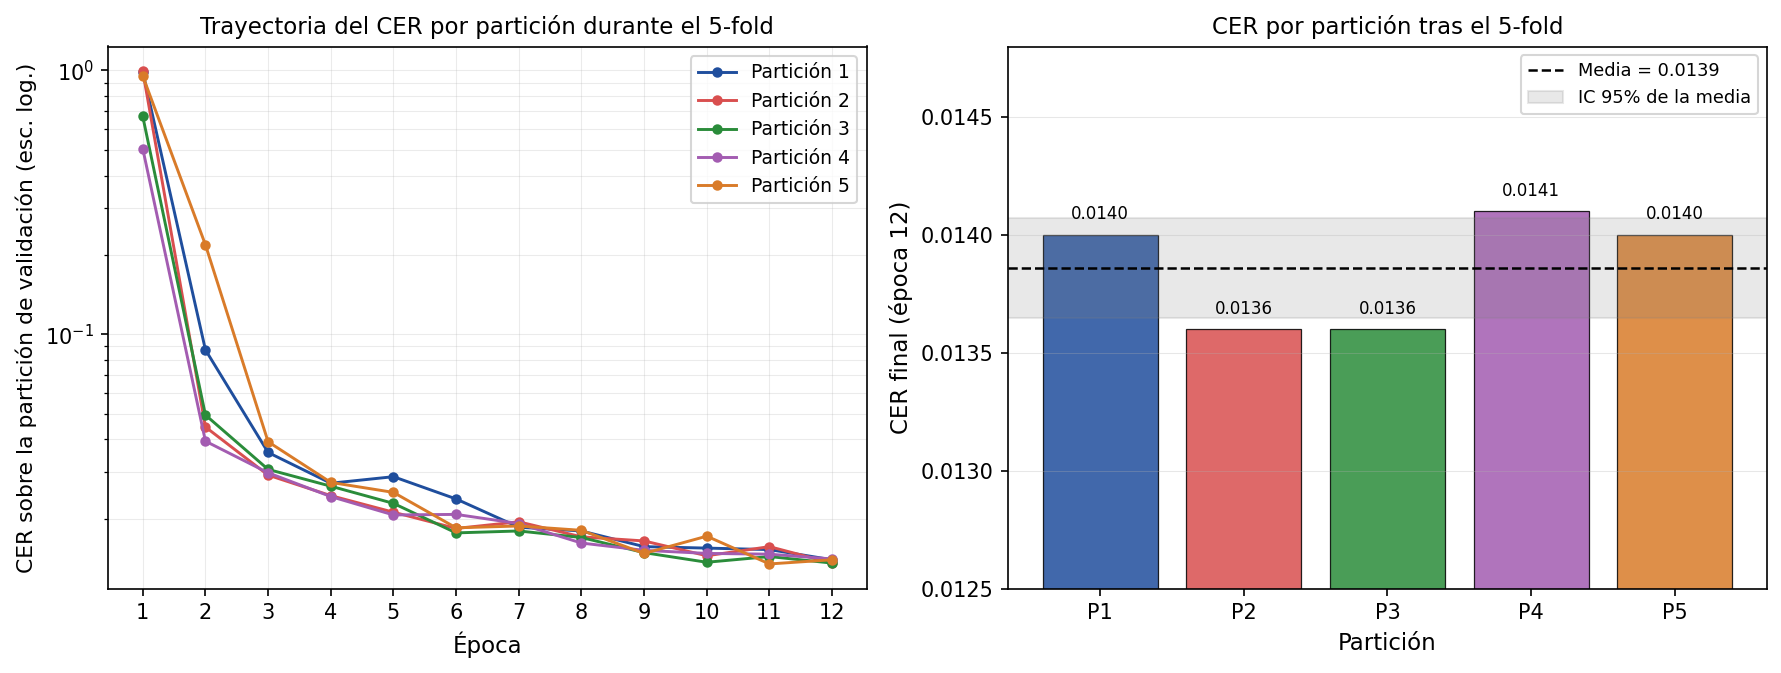
\includegraphics[width=\textwidth]{Graphics/cv_5fold.png}
	\caption{Validación cruzada de cinco particiones estratificadas por fuente. El panel izquierdo muestra la trayectoria del CER por época sobre la partición de validación correspondiente a cada repetición, en escala logarítmica. El panel derecho muestra el CER final tras doce épocas para cada partición, con la media (línea discontinua) y el intervalo de confianza al 95\,\% de la media (banda gris).}
	\label{fig:cv-5fold}
\end{figure}

El CER final de las cinco particiones cae en el intervalo $[0{,}0136;\ 0{,}0141]$, con media de 0,0138, desviación típica entre particiones de 0,00024 y coeficiente de variación de 1,7\,\%. La consistencia entre particiones indica que el rendimiento del modelo no depende de la partición aleatoria concreta del \textit{corpus}. La tabla~\ref{tab:cv-resumen} reporta el resumen agregado de las cinco métricas del protocolo de evaluación sobre las cinco repeticiones del experimento.

\begin{table}[!htbp]
	\centering
	\caption{Resumen agregado del experimento de validación cruzada de cinco particiones estratificadas por fuente. La columna \emph{Std} reporta la desviación típica entre particiones; las columnas \emph{Mín} y \emph{Máx} reportan el rango observado; la columna \emph{IC 95\,\%} reporta el intervalo de confianza al 95\,\% de la media de las cinco mediciones.}
	\label{tab:cv-resumen}
	\begin{tabular}{lccccc}
		\toprule
		\textbf{Métrica} & \textbf{Media} & \textbf{Std} & \textbf{Mín} & \textbf{Máx} & \textbf{IC 95\,\%} \\
		\midrule
		CER                  & 0,0138 & 0,00024 & 0,0135 & 0,0141 & $[0{,}0135,\ 0{,}0140]$ \\
		WER                  & 0,0490 & 0,00111 & 0,0472 & 0,0506 & $[0{,}0477,\ 0{,}0504]$ \\
		Exactitud por línea  & 0,7891 & 0,00653 & 0,7802 & 0,7991 & $[0{,}7810,\ 0{,}7972]$ \\
		Char-F1              & 0,9892 & 0,00022 & 0,9889 & 0,9895 & $[0{,}9890,\ 0{,}9895]$ \\
		BLEU-4 (carácter)    & 0,9746 & 0,00054 & 0,9738 & 0,9752 & $[0{,}9739,\ 0{,}9752]$ \\
		\bottomrule
	\end{tabular}
\end{table}

Los valores de la tabla~\ref{tab:cv-resumen} son sistemáticamente menos favorables que los del entrenamiento principal porque cada repetición de la validación cruzada entrena el modelo durante doce épocas sobre cuatro quintas partes del \textit{corpus}, frente a treinta épocas sobre nueve décimas partes del \textit{corpus} del entrenamiento principal. La comparación pertinente entre los dos protocolos no se refiere al nivel absoluto del CER sino a su variabilidad: la desviación típica del CER entre particiones, equivalente al 1,7\,\% de la media, confirma que el rendimiento del modelo no es accidente de una partición concreta.

El experimento LOFO produjo un CER promedio sobre las fuentes que quedan fuera de 0,0192, con intervalo de confianza al 95\,\% de $[0{,}0125,\ 0{,}0259]$. La degradación respecto al CER \textit{in-sample} de 0,0106 fue de 0,0086, valor inferior al umbral de 0,05 que el protocolo considera tolerable. La figura~\ref{fig:lofo-por-fuente} compara, para cada una de las nueve fuentes, el CER \textit{in-sample} (cuando la fuente sí participó en el entrenamiento) frente al CER LOFO (cuando la fuente quedó fuera).

\begin{figure}[!htbp]
	\centering
	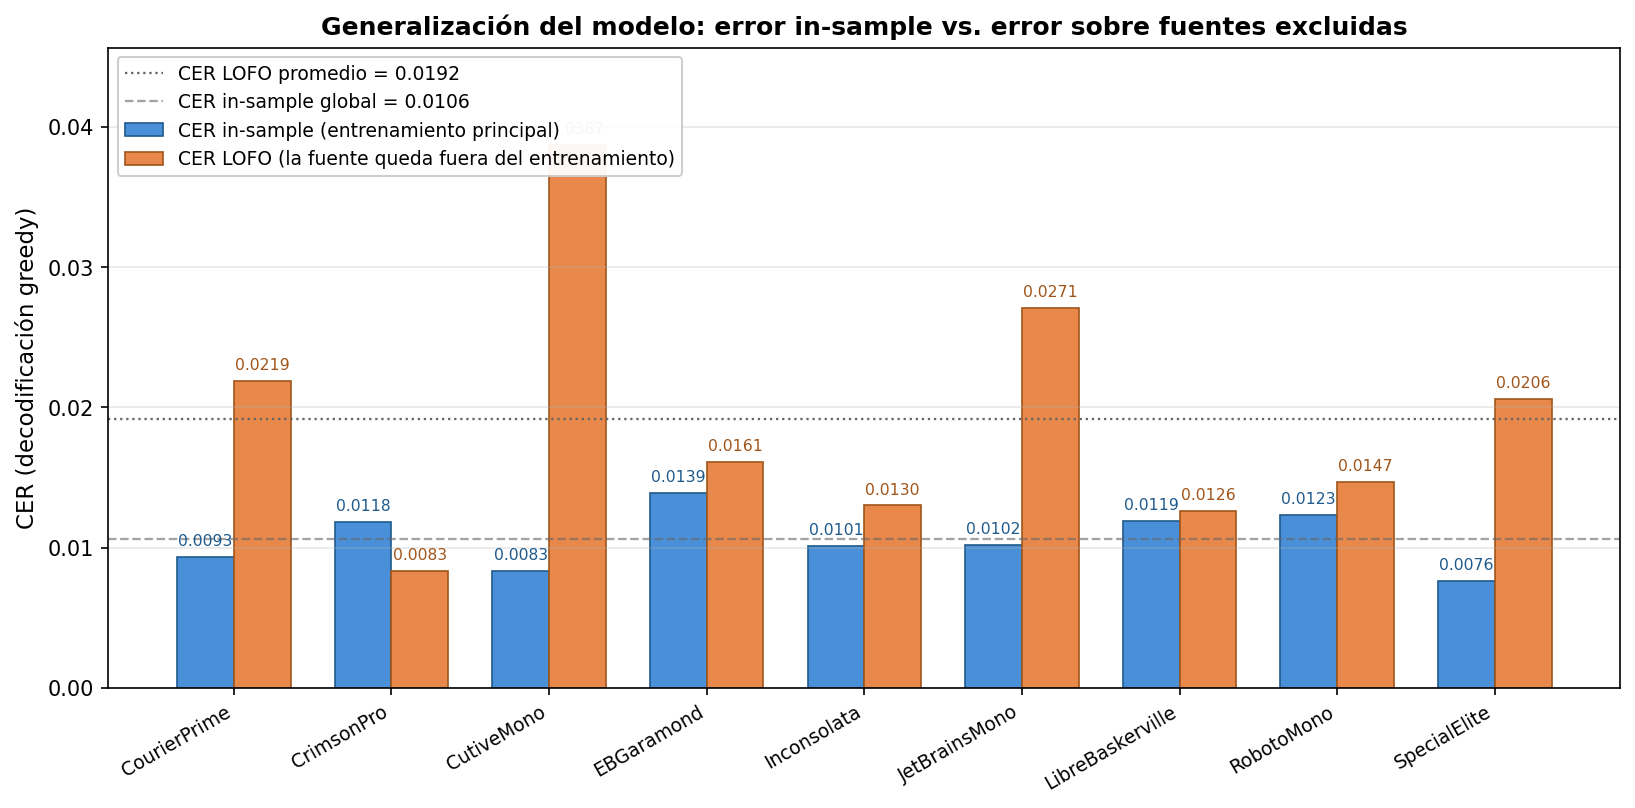
\includegraphics[width=\textwidth]{Graphics/lofo_por_fuente.png}
	\caption{Comparación del CER \textit{in-sample} (azul) y el CER LOFO (naranja) para cada una de las nueve fuentes del \textit{corpus} original. La línea discontinua marca el CER \textit{in-sample} global (0,0106) y la línea punteada marca el CER LOFO promedio (0,0192). La fuente con menor degradación es CrimsonPro y la fuente con mayor degradación es CutiveMono.}
	\label{fig:lofo-por-fuente}
\end{figure}

El comportamiento es marcadamente heterogéneo. CrimsonPro, LibreBaskerville e Inconsolata muestran degradaciones inferiores a 0,003 puntos, lo que indica que el modelo aprende a leerlas adecuadamente a partir de las restantes fuentes serif o monoespaciadas del \textit{corpus}. En el extremo opuesto, CutiveMono pasa de un CER \textit{in-sample} de 0,0083 a un CER LOFO de 0,0387, lo que sugiere que esta tipografía presenta rasgos que las restantes fuentes del \textit{corpus} cubren mal. JetBrainsMono y SpecialElite siguen patrones intermedios.

% -----------------------------------------------------------------------------
\section{Adaptación mediante \textit{fine-tuning}}
\label{sec:fine-tuning}

La etapa de \textit{fine-tuning} parte del modelo de la fase principal y continúa el entrenamiento sobre un \textit{corpus} con seis fuentes tipográficas adicionales. La ampliación responde a una observación práctica: durante la evaluación del modelo sobre documentos de prueba con tipografías serif que el entrenamiento principal no cubría, el equipo detectó errores sistemáticos sobre caracteres con remates que las tres serif del \textit{corpus} original representaban poco. La ampliación del repertorio tipográfico es la respuesta directa al objetivo, que el capítulo~\ref{chap:intro} declara, de maximizar la generalización del modelo frente a tipografías arbitrarias.

Las seis fuentes que el corpus extendido añade son Lora, Merriweather, Palatino, SourceSerif4, Georgia y Times. El conjunto refuerza la familia serif del \textit{corpus} original con tipografías de uso amplio en publicaciones modernas y en sistemas operativos comerciales. La generación del \textit{corpus} extendido sigue el procedimiento que el capítulo~\ref{chap:corpus} describe, con la única diferencia del catálogo tipográfico.

\subsection{Análisis exploratorio del \textit{corpus} extendido}
\label{subsec:eda-extendido}

El \textit{corpus} extendido pasa por el mismo procedimiento de análisis exploratorio que la sección~\ref{sec:eda-corpus} del capítulo~\ref{chap:corpus} aplicó al \textit{corpus} de entrenamiento. La caracterización del \textit{corpus} extendido es necesaria para confirmar que las propiedades de diseño que sostienen la generación se mantienen tras la ampliación del catálogo tipográfico, y para verificar que las nuevas fuentes siguen cumpliendo la restricción de la función de pérdida CTC. La figura~\ref{fig:eda-dashboard-extendido} reúne las visualizaciones del análisis.

\begin{figure}[!htbp]
	\centering
	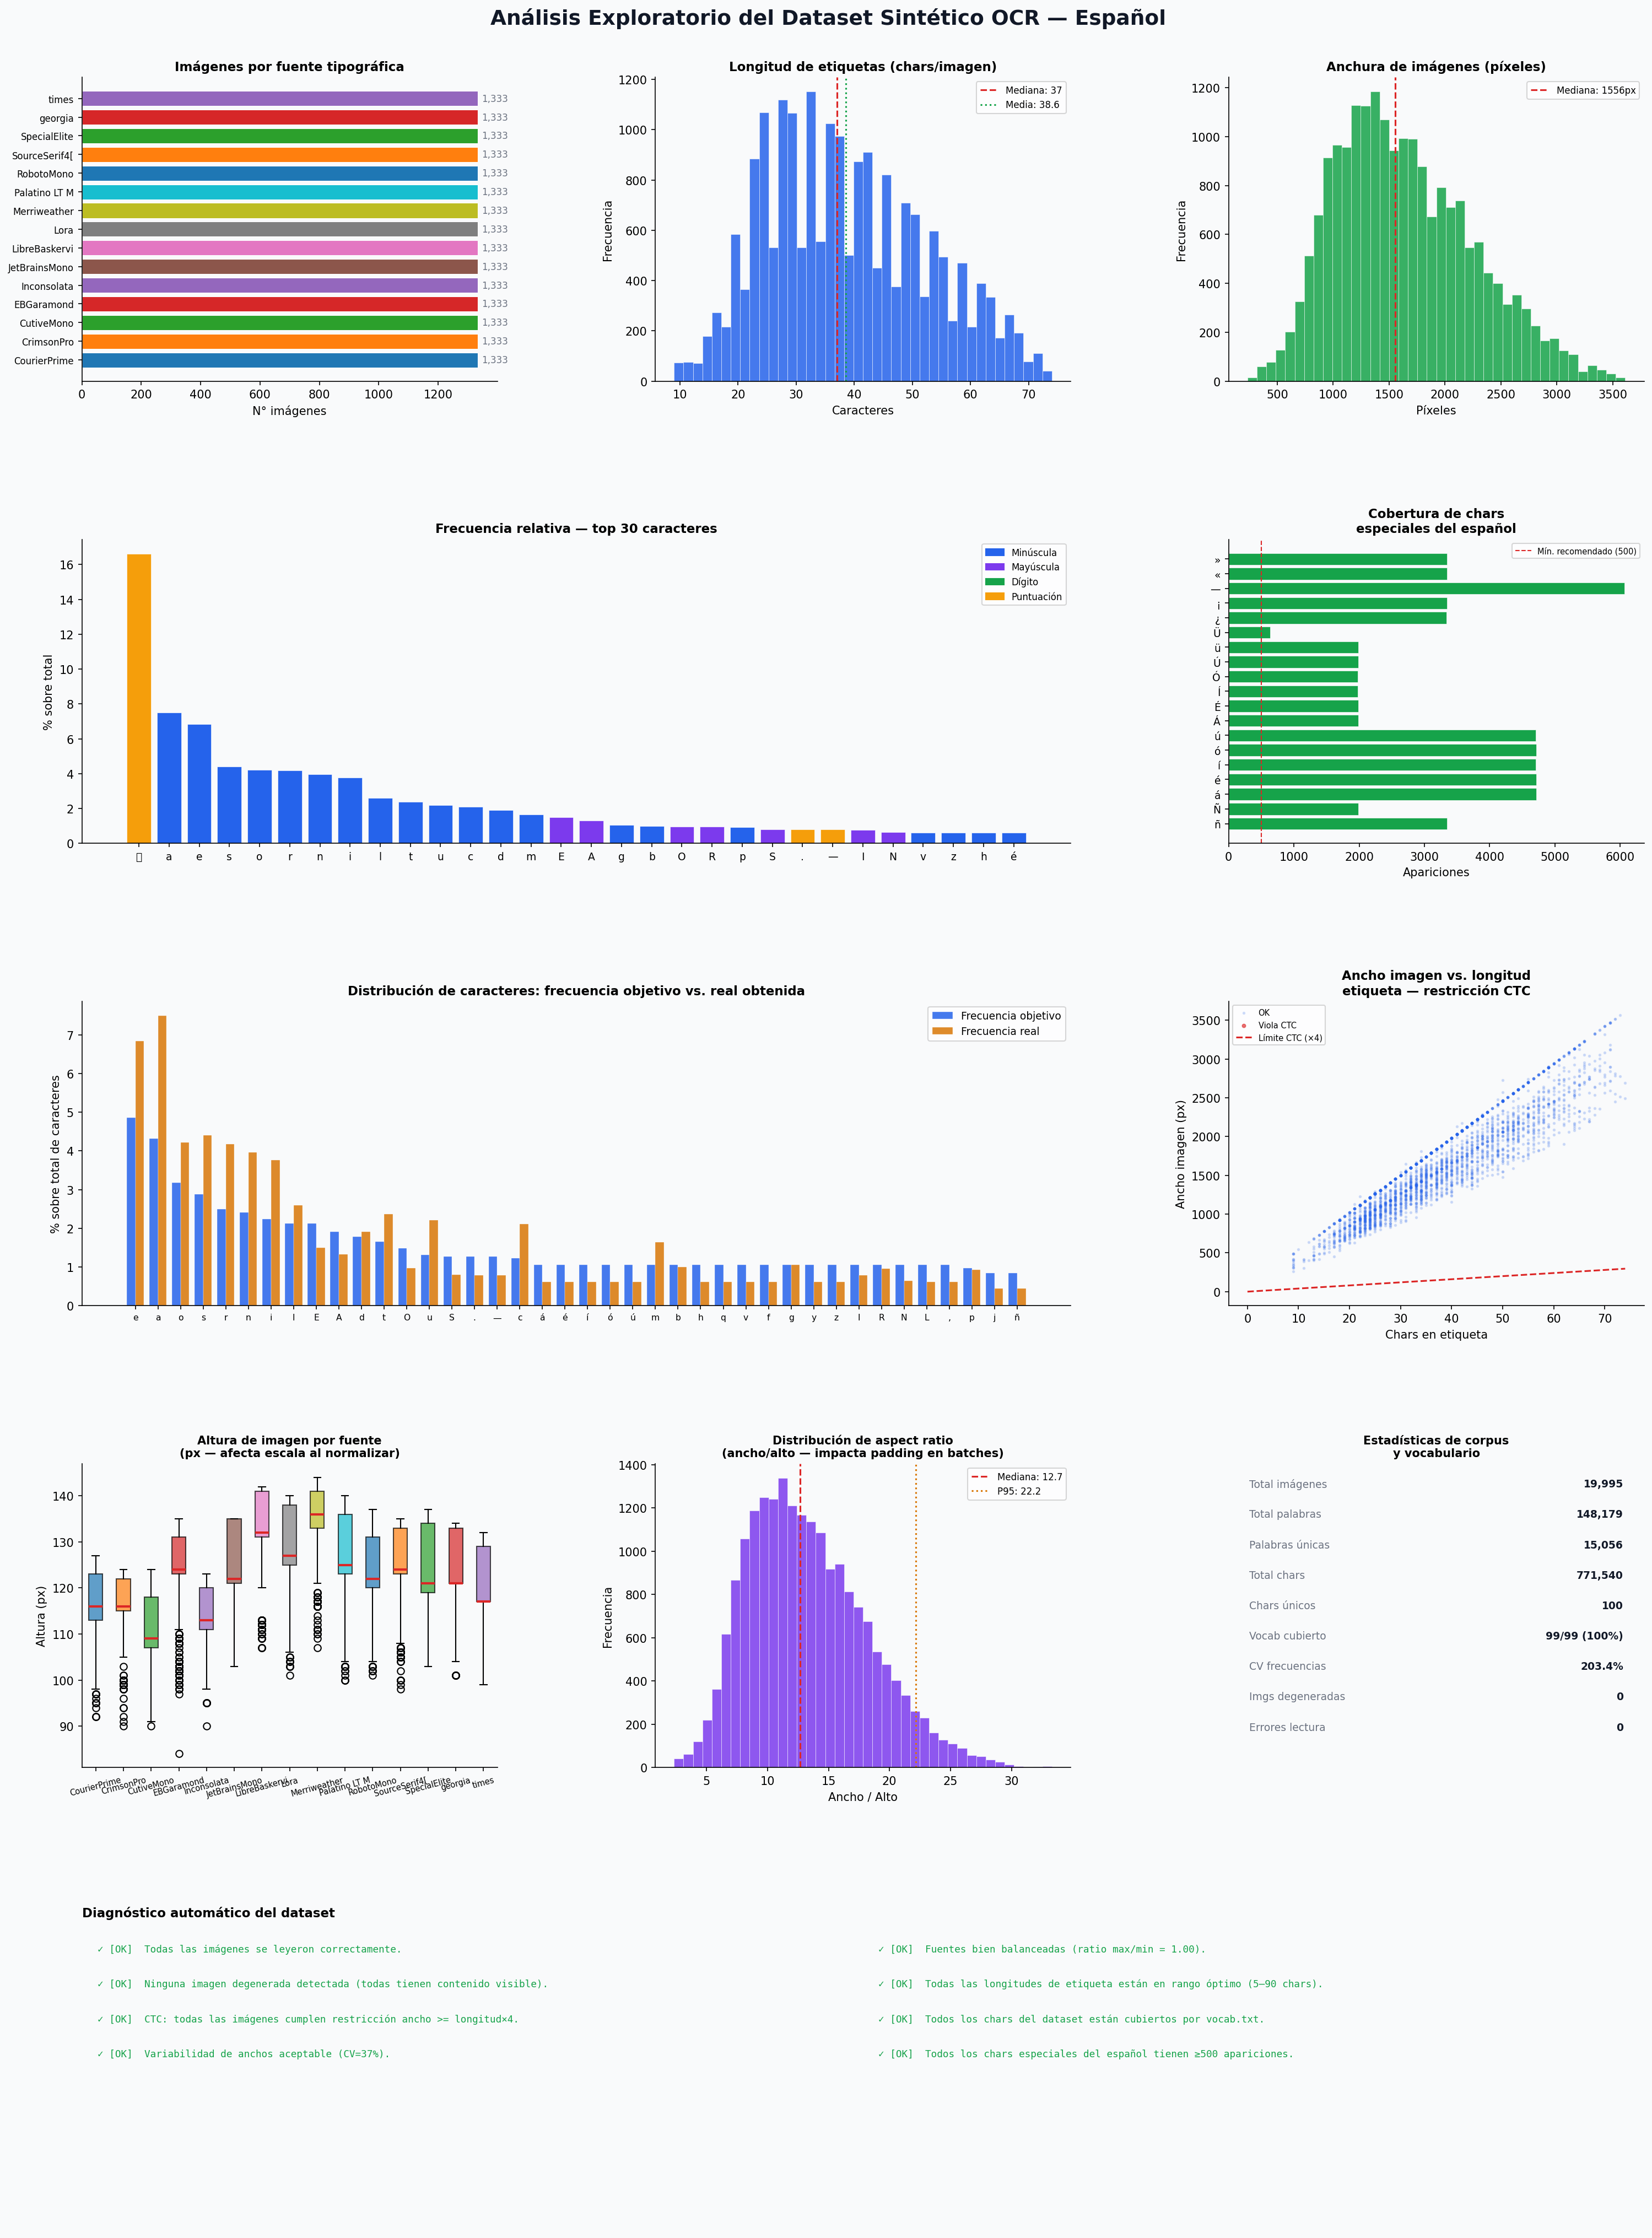
\includegraphics[width=0.85\textwidth]{Graphics/eda_dashboard_extendido.png}
	\caption{Análisis exploratorio del \textit{corpus} sintético extendido para la etapa de \textit{fine-tuning}, con 19\,995 imágenes que el generador produce a partir de las quince fuentes tipográficas (las nueve del \textit{corpus} original más las seis que se añaden en esta etapa). El panel reúne las distribuciones de imágenes por fuente, longitudes de etiqueta, anchos, frecuencias de caracteres, cobertura del vocabulario español, cumplimiento de la restricción CTC, alturas por fuente y aspect ratio de las imágenes.}
	\label{fig:eda-dashboard-extendido}
\end{figure}

El \textit{corpus} extendido reúne 19\,995 imágenes con un reparto perfectamente uniforme entre las quince fuentes, 1\,333 imágenes por cada una, y cociente máximo--mínimo igual a la unidad. La reducción de la cuota por fuente respecto al \textit{corpus} original, donde cada fuente aportaba 2\,222 imágenes, es la consecuencia directa de mantener el tamaño global del \textit{corpus} constante mientras el catálogo tipográfico crece. La decisión de no aumentar el volumen global respeta la práctica habitual del \textit{fine-tuning}, que opera con cantidades de datos del mismo orden que el entrenamiento principal y no requiere ampliar el volumen agregado.

Las longitudes de etiqueta presentaron media de 38,6 caracteres, mediana de 37, rango entre 9 y 74 y desviación típica de 13,8, con percentiles 5, 25, 75 y 95 en 19, 28, 48 y 64 caracteres, respectivamente. Los valores reproducen casi exactamente la distribución del \textit{corpus} original, lo que indica que el algoritmo de generación de cadenas balanceadas que el capítulo~\ref{chap:corpus} describe es robusto frente al cambio del repertorio tipográfico.

Las dimensiones de imagen presentaron media de ancho de 1\,639 píxeles, mediana de 1\,556 píxeles, rango entre 234 y 3\,612 píxeles y coeficiente de variación del 37,5\,\%. La media de altura fue de 123 píxeles, con rango entre 84 y 144 píxeles. La pequeña reducción del ancho medio respecto al \textit{corpus} original (1\,704 píxeles) refleja la incorporación de fuentes serif modernas con paso tipográfico más compacto que las monoespacio dominantes del \textit{corpus} original. La verificación de la restricción CTC sobre el \textit{corpus} extendido confirmó que ninguna de las 19\,995 imágenes la viola, en línea con el resultado equivalente sobre el \textit{corpus} de entrenamiento.

La cobertura del vocabulario fue total: el \textit{corpus} extendido contiene los cien símbolos del vocabulario del sistema. El \textit{corpus} reúne 771\,540 caracteres en 148\,179 palabras, de las cuales 15\,056 son únicas. El coeficiente de variación de las frecuencias de caracteres alcanzó el 203,4\,\%, valor casi idéntico al del \textit{corpus} original y consistente con la ley de Zipf del lenguaje natural. Los caracteres específicos del español formal mantienen todos la cobertura por encima del umbral mínimo de 500 apariciones, con la eñe en 3\,348 apariciones, las comillas angulares en 3\,346 y 3\,343, la raya de diálogo en 6\,061 y los signos de apertura de interrogación y exclamación por encima de 3\,300 cada uno. Tres símbolos genéricos quedan por debajo del umbral, los mismos que en el \textit{corpus} original: el corchete derecho (89 apariciones), el corchete izquierdo (85) y la almohadilla (81). El criterio que la sección~\ref{sec:eda-corpus} expuso aplica también aquí: los tres no figuran entre los caracteres específicos del español y la cobertura mínima del vocabulario del idioma resulta satisfactoria.

El análisis exploratorio confirma que el \textit{corpus} extendido conserva todas las propiedades de diseño del \textit{corpus} original: uniformidad entre fuentes, distribución de longitudes en rango operativo, cobertura completa del vocabulario, todos los caracteres del español por encima del umbral mínimo, y respeto de la restricción CTC. La única diferencia, por diseño, está en la cuota por fuente, que disminuye a la mitad por el incremento del catálogo de nueve a quince fuentes. La caracterización valida el \textit{corpus} extendido como entrada apta para la etapa de \textit{fine-tuning}.

\subsection{Protocolo de \textit{fine-tuning}}
\label{subsec:protocolo-finetune}

El protocolo de \textit{fine-tuning} reutiliza la configuración del entrenamiento principal con las diferencias que la tabla~\ref{tab:diff-finetune} resume.

\begin{table}[!htbp]
	\centering
	\caption{Diferencias de configuración entre el entrenamiento principal y la etapa de \textit{fine-tuning}.}
	\label{tab:diff-finetune}
	\scriptsize
	\begin{tabular}{lcc}
		\toprule
		\textbf{Hiperparámetro} & \textbf{Entrenamiento principal} & \textbf{\textit{Fine-tuning}} \\
		\midrule
		Punto de partida & pesos inicializados (Xavier) & mejor \textit{checkpoint} de la fase principal \\
		Épocas & 30 & 20 \\
		Tasa de aprendizaje máxima & $3 \times 10^{-4}$ & $5 \times 10^{-5}$ \\
		Recorte de gradiente (norma máx.) & 5,0 & 3,0 \\
		Catálogo tipográfico (fuentes) & 9 & 15 \\
		\bottomrule
	\end{tabular}
\end{table}

La reducción de la tasa de aprendizaje a aproximadamente un sexto y la del recorte de gradiente reflejan la práctica habitual de continuación desde un punto de control preentrenado: el modelo parte ya de una buena solución y conviene evitar pasos demasiado grandes que la destruyan. El conjunto de hiperparámetros restante coincide con el del entrenamiento principal. La figura~\ref{fig:curvas-finetuning} muestra la trayectoria de las tres métricas de error sobre el conjunto de validación a lo largo de las veinte épocas del \textit{fine-tuning}.

\begin{figure}[!htbp]
	\centering
	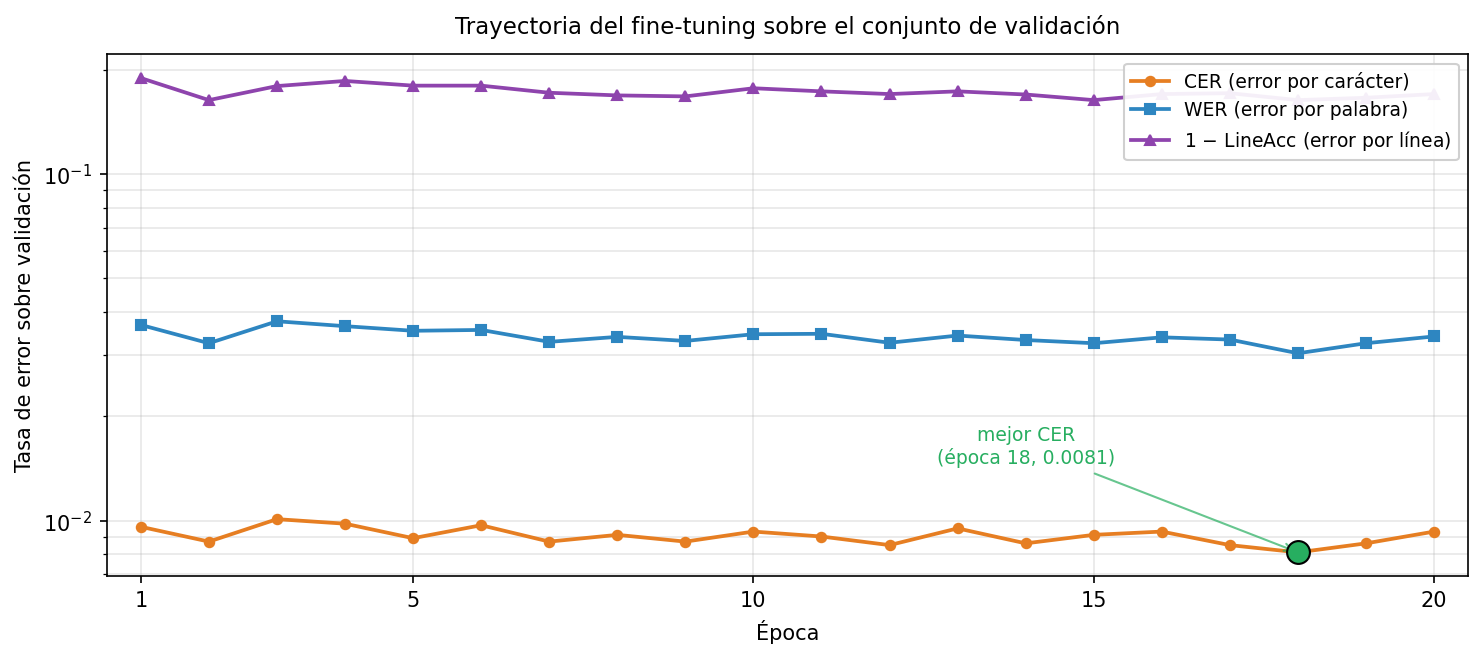
\includegraphics[width=\textwidth]{Graphics/curvas_finetuning.png}
	\caption{Trayectoria de las tres métricas de error sobre el conjunto de validación sintética con decodificación \textit{greedy}, a lo largo de las veinte épocas del \textit{fine-tuning} sobre el \textit{corpus} extendido. El eje vertical, en escala logarítmica, comparte el rango con la figura~\ref{fig:curvas-entrenamiento} del entrenamiento principal para facilitar la comparación visual. El régimen es estacionario desde la primera época, con oscilaciones en un entorno cerrado en torno a CER 0,009, WER 0,034 y tasa de error por línea 0,17. La ausencia de tendencia descendente es esperable, ya que el \textit{fine-tuning} parte del mejor \textit{checkpoint} del entrenamiento principal, que el modelo no podía mejorar de forma apreciable sin un cambio de dominio o de capacidad. El marcador verde señala el mejor CER, que el modelo alcanza en la época dieciocho con valor 0,0081.}
	\label{fig:curvas-finetuning}
\end{figure}

La tabla~\ref{tab:comparativa-finetune} compara las métricas globales antes y después del \textit{fine-tuning}.

\begin{table}[!htbp]
	\centering
	\caption{Métricas globales antes y después del \textit{fine-tuning} sobre el conjunto de validación correspondiente. La columna de variación reporta la reducción porcentual sobre el CER y el WER.}
	\label{tab:comparativa-finetune}
	\begin{tabular}{lccc}
		\toprule
		\textbf{Métrica} & \textbf{Principal (9 fuentes)} & \textbf{\textit{Fine-tuning} (15 fuentes)} & \textbf{Variación} \\
		\midrule
		CER             & 0,0106 & 0,0088 & $-17{,}\%$ \\
		WER             & 0,0374 & 0,0331 & $-12{,}\%$ \\
		Exactitud por línea & 0,8269 & 0,8304 & $+0{,}35$~pp \\
		\bottomrule
	\end{tabular}
\end{table}

El modelo final, sobre la validación extendida de quince fuentes, alcanza un CER del 0{,}88\,\%, valor consistente con el rango del entrenamiento principal sobre las nueve fuentes originales (CER del 1{,}06\,\%). Las dos cifras corresponden a distribuciones de validación distintas y una comparación isodistribuida estricta exigiría medir el modelo principal sobre la validación extendida; la subsección~\ref{subsec:lofo-post-ft} reporta la comparación rigurosa entre ambos modelos sobre un mismo protocolo experimental, que cuantifica el efecto del \textit{fine-tuning} sobre la generalización tipográfica. La prueba de Kruskal-Wallis sobre las quince fuentes del \textit{corpus} extendido no rechaza la hipótesis de igualdad de distribuciones entre fuentes ($H = 17{,}04$, $p = 0{,}254$), lo que indica que el modelo, tras el \textit{fine-tuning}, alcanza una uniformidad de rendimiento entre fuentes consistente con la del entrenamiento original. La tabla~\ref{tab:cer-por-fuente-finetune} reporta el CER de cada una de las quince fuentes.

\begin{table}[!htbp]
	\centering
	\caption{CER por fuente tipográfica tras el \textit{fine-tuning} sobre el \textit{corpus} extendido. La columna \emph{Std} reporta la desviación típica del CER por muestra dentro de la fuente. Las seis fuentes que se añaden en esta etapa aparecen en negrita.}
	\label{tab:cer-por-fuente-finetune}
	\begin{tabular}{lccc}
		\toprule
		\textbf{Fuente} & \textbf{CER} & \textbf{Std} & \textbf{IC 95\,\%} \\
		\midrule
		CourierPrime      & 0,0125 & 0,0387 & $[0{,}0065,\ 0{,}0200]$ \\
		CrimsonPro        & 0,0042 & 0,0125 & $[0{,}0022,\ 0{,}0066]$ \\
		CutiveMono        & 0,0062 & 0,0205 & $[0{,}0031,\ 0{,}0100]$ \\
		EBGaramond        & 0,0095 & 0,0233 & $[0{,}0062,\ 0{,}0135]$ \\
		Inconsolata       & 0,0122 & 0,0393 & $[0{,}0064,\ 0{,}0191]$ \\
		JetBrainsMono     & 0,0134 & 0,0454 & $[0{,}0068,\ 0{,}0223]$ \\
		LibreBaskerville  & 0,0067 & 0,0236 & $[0{,}0031,\ 0{,}0114]$ \\
		\textbf{Lora}     & 0,0080 & 0,0252 & $[0{,}0038,\ 0{,}0127]$ \\
		\textbf{Merriweather} & 0,0090 & 0,0459 & $[0{,}0025,\ 0{,}0184]$ \\
		\textbf{Palatino} & 0,0106 & 0,0420 & $[0{,}0045,\ 0{,}0192]$ \\
		RobotoMono        & 0,0106 & 0,0367 & $[0{,}0054,\ 0{,}0177]$ \\
		\textbf{SourceSerif4} & 0,0053 & 0,0153 & $[0{,}0028,\ 0{,}0083]$ \\
		SpecialElite      & 0,0064 & 0,0234 & $[0{,}0030,\ 0{,}0109]$ \\
		\textbf{Georgia}  & 0,0097 & 0,0291 & $[0{,}0055,\ 0{,}0154]$ \\
		\textbf{Times}    & 0,0072 & 0,0291 & $[0{,}0031,\ 0{,}0130]$ \\
		\bottomrule
	\end{tabular}
\end{table}

El análisis de los errores de carácter más frecuentes que el modelo final produce identifica dos patrones predominantes. El primero es la confusión entre signos de puntuación visualmente similares, con la coma que el modelo confunde con el punto como el error más frecuente. El segundo es la omisión de tildes, que confunde la vocal con tilde con su contrapartida sin tilde. Los dos patrones son consistentes con la dificultad de los caracteres que intervienen, que difieren por rasgos de pocos píxeles en tipografías de cuerpo pequeño.

% -----------------------------------------------------------------------------
\section{Evaluación final sobre el conjunto de prueba}
\label{sec:test-set}

La evaluación final del sistema descansa sobre un conjunto de prueba independiente que el protocolo reserva para una única medición, después de la etapa de \textit{fine-tuning} que la sección~\ref{sec:fine-tuning} describe. La medición sobre este conjunto constituye la estimación insesgada del rendimiento del modelo desplegado: el conjunto de prueba no participa en la selección del \textit{checkpoint}, no contribuye a las decisiones de hiperparámetros y el desarrollo no lo observa más de una vez.

La decisión de aplicar la evaluación final únicamente después del \textit{fine-tuning}, y no al término del entrenamiento principal, responde a dos consideraciones metodológicas. La primera es que el modelo que el sistema despliega corresponde al modelo posterior al \textit{fine-tuning}; una evaluación intermedia tras el entrenamiento principal habría producido la métrica de un modelo que no llega a producción, sin valor operativo para los resultados que el documento reporta. La segunda es que reutilizar el conjunto de prueba en dos momentos del desarrollo, uno tras el entrenamiento principal y otro tras el \textit{fine-tuning}, habría introducido un sesgo de selección sobre la decisión misma de continuar con la adaptación: la observación del primer número habría podido influir en el resto del proceso, lo que invalidaría la segunda medición como estimador insesgado. La política de uso único del conjunto de prueba es la práctica habitual en aprendizaje automático precisamente por esta razón. Durante el desarrollo, la validación cruzada estratificada por fuente y el experimento de exclusión de una fuente que la subsección~\ref{subsec:cv-lofo} describe cumplieron el papel de cuantificación de la generalización sin consumir el presupuesto del conjunto de prueba.

\subsection{Composición del conjunto de prueba}
\label{subsec:test-composicion}

El generador del \textit{corpus} produjo 1\,995 imágenes a partir de las quince fuentes tipográficas del repertorio extendido, con un reparto perfectamente uniforme de 133 imágenes por fuente y un cociente entre la frecuencia máxima y la mínima igual a la unidad. El procedimiento de generación es idéntico al que el capítulo~\ref{chap:corpus} describe para el \textit{corpus} de entrenamiento, con una sola diferencia: la semilla aleatoria que controla el muestreo de cadenas a partir del \textit{corpus} textual de Project Gutenberg toma un valor distinto del que la generación del \textit{corpus} de entrenamiento empleó. El cambio de semilla garantiza por construcción que ninguna cadena del conjunto de prueba coincida con una del entrenamiento o la validación. La longitud media de las cadenas del conjunto de prueba es de 38,7 caracteres, en línea con la del \textit{corpus} de entrenamiento que el capítulo~\ref{chap:corpus} reporta.

\subsection{Resultados globales}
\label{subsec:test-global}

La tabla~\ref{tab:test-global} reporta las métricas principales sobre el conjunto de prueba con decodificación \textit{greedy} sobre el modelo final tras el \textit{fine-tuning}, con intervalos de confianza al 95\,\% por \textit{bootstrap} con diez mil remuestreos.

\begin{table}[!htbp]
	\centering
	\caption{Resultados del modelo final sobre el conjunto de prueba independiente de 1\,995 imágenes. Decodificación \textit{greedy} sobre el modelo posterior a la etapa de \textit{fine-tuning}. El procedimiento \textit{bootstrap} con diez mil remuestreos produce los intervalos de confianza al 95\,\%. La métrica BLEU-4 es una métrica agregada del conjunto y no admite intervalo de confianza por remuestreo de muestras individuales.}
	\label{tab:test-global}
	\begin{tabular}{lccc}
		\toprule
		\textbf{Métrica}     & \textbf{Media} & \textbf{Std} & \textbf{IC 95\,\%} \\
		\midrule
		CER                  & 0,0428 & 0,0469 & $[0{,}0407,\ 0{,}0448]$ \\
		WER                  & 0,0973 & 0,1333 & $[0{,}0916,\ 0{,}1032]$ \\
		Exactitud por línea  & 0,3739 & 0,4840 & $[0{,}3524,\ 0{,}3950]$ \\
		Char-F1              & 0,9793 & 0,0222 & $[0{,}9783,\ 0{,}9803]$ \\
		BLEU-4 (carácter)    & 0,9625 & ---    & --- \\
		\bottomrule
	\end{tabular}
\end{table}

El CER del 4,28\,\% sobre el conjunto de prueba es superior al CER del 0,88\,\% que el conjunto de validación reportó tras el \textit{fine-tuning}. Tres factores combinados explican la diferencia. El primero es la selección del \textit{checkpoint} durante el entrenamiento: el protocolo guarda en cada época el modelo con menor CER sobre validación, lo que introduce un sesgo optimista sobre la métrica de validación. El segundo es el origen de las cadenas: el protocolo obtiene el conjunto de validación por partición aleatoria del \textit{corpus} de entrenamiento, mientras que el conjunto de prueba parte de un muestreo independiente del mismo \textit{corpus} textual de Project Gutenberg con una semilla distinta, lo que produce material léxico que el modelo no encontró durante el entrenamiento. El tercero es la política de uso único: el protocolo evalúa el conjunto de prueba una sola vez sobre el modelo final, sin posibilidad de selección posterior. La estimación de prueba constituye, por estos tres motivos, el indicador insesgado del rendimiento que cabe esperar del modelo en condiciones operativas sobre material sintético comparable. El CER del 4,28\,\% sitúa al sistema en un rango competitivo con los motores OCR para texto impreso en español según la discusión del estado del arte que el capítulo~\ref{chap:estado-arte} ofrece, y la exactitud por línea próxima al 37\,\% indica que más de una de cada tres líneas recibe transcripción sin error alguno.

\subsection{Resultados por fuente tipográfica}
\label{subsec:test-por-fuente}

La tabla~\ref{tab:test-por-fuente} reporta el CER, la desviación típica del CER por muestra, la exactitud por línea y el intervalo de confianza al 95\,\% sobre el CER, para cada una de las quince fuentes del conjunto de prueba.

\begin{table}[!htbp]
	\centering
	\caption{CER, desviación típica del CER por muestra, exactitud por línea e intervalo de confianza al 95\,\% sobre el CER por fuente tipográfica, sobre el conjunto de prueba de 1\,995 imágenes (133 por fuente). Decodificación \textit{greedy} sobre el modelo final tras \textit{fine-tuning}. Las seis fuentes en negrita son las que el \textit{fine-tuning} añadió al \textit{corpus} original.}
	\label{tab:test-por-fuente}
	\begin{tabular}{lcccc}
		\toprule
		\textbf{Fuente} & \textbf{CER} & \textbf{Std} & \textbf{LineAcc} & \textbf{IC 95\,\%} \\
		\midrule
		CourierPrime          & 0,0214 & 0,0315 & 0,5940 & $[0{,}0163,\ 0{,}0268]$ \\
		CrimsonPro            & 0,0556 & 0,0530 & 0,3008 & $[0{,}0469,\ 0{,}0646]$ \\
		CutiveMono            & 0,0170 & 0,0309 & 0,6541 & $[0{,}0120,\ 0{,}0225]$ \\
		EBGaramond            & 0,0597 & 0,0579 & 0,2632 & $[0{,}0501,\ 0{,}0698]$ \\
		Inconsolata           & 0,0291 & 0,0424 & 0,5188 & $[0{,}0223,\ 0{,}0366]$ \\
		JetBrainsMono         & 0,0200 & 0,0275 & 0,5489 & $[0{,}0156,\ 0{,}0248]$ \\
		LibreBaskerville      & 0,0422 & 0,0422 & 0,3233 & $[0{,}0354,\ 0{,}0496]$ \\
		\textbf{Lora}         & 0,0572 & 0,0457 & 0,2180 & $[0{,}0497,\ 0{,}0651]$ \\
		\textbf{Merriweather} & 0,0552 & 0,0493 & 0,2632 & $[0{,}0469,\ 0{,}0635]$ \\
		\textbf{Palatino}     & 0,0514 & 0,0468 & 0,3008 & $[0{,}0437,\ 0{,}0594]$ \\
		RobotoMono            & 0,0167 & 0,0280 & 0,6316 & $[0{,}0122,\ 0{,}0215]$ \\
		\textbf{SourceSerif4} & 0,0514 & 0,0510 & 0,3308 & $[0{,}0430,\ 0{,}0602]$ \\
		SpecialElite          & 0,0521 & 0,0550 & 0,2406 & $[0{,}0434,\ 0{,}0621]$ \\
		\textbf{Georgia}      & 0,0601 & 0,0461 & 0,1880 & $[0{,}0524,\ 0{,}0681]$ \\
		\textbf{Times}        & 0,0523 & 0,0404 & 0,2331 & $[0{,}0456,\ 0{,}0593]$ \\
		\bottomrule
	\end{tabular}
\end{table}

La prueba de Kruskal-Wallis~\cite{kruskal1952ranks} sobre el CER entre las quince fuentes rechaza la hipótesis de igualdad de distribuciones con $H = 280{,}90$ y un valor de probabilidad inferior a $10^{-50}$. El rechazo contrasta con el resultado de las pruebas equivalentes sobre los conjuntos de validación del entrenamiento principal ($H = 11{,}93$, $p = 0{,}154$) y del \textit{fine-tuning} ($H = 17{,}04$, $p = 0{,}254$) que las secciones~\ref{sec:resultados-entrenamiento} y~\ref{sec:fine-tuning} reportan, y refleja que la evaluación sobre material léxico independiente del entrenamiento expone diferencias sistemáticas de dificultad entre familias tipográficas que la evaluación sobre material léxico compartido enmascara.

El comportamiento por fuente sigue un patrón coherente con la estructura del catálogo tipográfico. Las cinco fuentes monoespaciadas (CourierPrime, CutiveMono, Inconsolata, JetBrainsMono y RobotoMono) alcanzan los CER más bajos del rango, entre 0,0167 y 0,0291, y exactitudes por línea entre el 52\,\% y el 66\,\%. Las nueve fuentes serif, tanto las del \textit{corpus} original (CrimsonPro, EBGaramond y LibreBaskerville) como las seis que el \textit{fine-tuning} incorporó (Lora, Merriweather, Palatino, SourceSerif4, Georgia y Times), junto con la fuente SpecialElite que simula máquina de escribir, presentan CER entre 0,0422 y 0,0601 y exactitudes por línea entre el 19\,\% y el 33\,\%. La diferencia sistemática refleja la mayor dificultad intrínseca de los rasgos con remates y de la variabilidad del trazo característica de las tipografías serif, frente a la uniformidad geométrica de las monoespaciadas. Las seis fuentes que el \textit{fine-tuning} incorporó alcanzan un rendimiento equiparable al de las tres fuentes serif del \textit{corpus} original (CER entre 0,051 y 0,060 frente a 0,042 y 0,060 respectivamente), lo que confirma que la etapa de adaptación cumplió el objetivo de incorporar el repertorio serif moderno al conocimiento del modelo sin desequilibrar el rendimiento entre fuentes históricamente cubiertas y fuentes recién incorporadas.

% -----------------------------------------------------------------------------
\subsection{Evaluación \textit{Leave-One-Font-Out} sobre el modelo final}
\label{subsec:lofo-post-ft}

El protocolo reaplica el experimento \textit{Leave-One-Font-Out}~\cite{etter2019synthrecipe} que la subsección~\ref{subsec:cv-lofo} introduce sobre el modelo final tras la etapa de \textit{fine-tuning}, ahora con el repertorio extendido de quince fuentes. El procedimiento es idéntico al del entrenamiento principal: cada repetición excluye una fuente del entrenamiento, adapta los pesos del modelo final durante diez épocas sobre el \textit{corpus} restante y mide el CER sobre la fuente que quedó fuera. La medición tiene dos propósitos. El primero es cuantificar la capacidad de generalización del modelo final a tipografías que el entrenamiento no observó. El segundo es proporcionar una comparación directa con el LOFO sobre el modelo principal de nueve fuentes, ya que ambos experimentos siguen un protocolo isodistribuido, en contraste con la comparación de validaciones que la sección~\ref{sec:fine-tuning} reportó sobre distribuciones distintas. La tabla~\ref{tab:lofo-post-ft} reporta los resultados de las quince repeticiones.

\begin{table}[!htbp]
	\centering
	\caption{Resultados del experimento \textit{Leave-One-Font-Out} sobre el modelo final tras el \textit{fine-tuning}. Cada fila corresponde a una repetición que excluye la fuente indicada del entrenamiento y la usa como conjunto de evaluación. El CER medio sobre las quince fuentes coincide en términos prácticos con el CER de validación del modelo final cuando ve todas las fuentes durante el entrenamiento.}
	\label{tab:lofo-post-ft}
	\small
	\begin{tabular}{lcccc}
		\toprule
		\textbf{Fuente excluida} & \textbf{CER} & \textbf{IC 95\,\%} & \textbf{WER} & \textbf{LineAcc} \\
		\midrule
		CourierPrime          & 0,0143 & $[0{,}0121,\ 0{,}0167]$ & 0,0487 & 0,7769 \\
		CrimsonPro            & 0,0059 & $[0{,}0048,\ 0{,}0071]$ & 0,0244 & 0,8651 \\
		CutiveMono            & 0,0205 & $[0{,}0179,\ 0{,}0233]$ & 0,0690 & 0,7023 \\
		EBGaramond            & 0,0058 & $[0{,}0047,\ 0{,}0069]$ & 0,0247 & 0,8685 \\
		Inconsolata           & 0,0096 & $[0{,}0079,\ 0{,}0114]$ & 0,0369 & 0,8118 \\
		JetBrainsMono         & 0,0140 & $[0{,}0118,\ 0{,}0163]$ & 0,0520 & 0,7646 \\
		LibreBaskerville      & 0,0072 & $[0{,}0060,\ 0{,}0085]$ & 0,0310 & 0,8326 \\
		Lora                  & 0,0068 & $[0{,}0057,\ 0{,}0080]$ & 0,0289 & 0,8440 \\
		Merriweather          & 0,0055 & $[0{,}0046,\ 0{,}0065]$ & 0,0250 & 0,8498 \\
		Palatino              & 0,0066 & $[0{,}0054,\ 0{,}0080]$ & 0,0284 & 0,8546 \\
		RobotoMono            & 0,0128 & $[0{,}0108,\ 0{,}0148]$ & 0,0495 & 0,7784 \\
		SourceSerif4          & 0,0063 & $[0{,}0052,\ 0{,}0073]$ & 0,0281 & 0,8388 \\
		SpecialElite          & 0,0078 & $[0{,}0064,\ 0{,}0092]$ & 0,0316 & 0,8370 \\
		Georgia               & 0,0068 & $[0{,}0056,\ 0{,}0080]$ & 0,0279 & 0,8395 \\
		Times                 & 0,0064 & $[0{,}0054,\ 0{,}0076]$ & 0,0263 & 0,8523 \\
		\midrule
		\textbf{Media}        & \textbf{0,0091} & \textbf{[0{,}0067,\ 0{,}0114]} & \textbf{0,0355} & \textbf{0,8211} \\
		\bottomrule
	\end{tabular}
\end{table}

El CER medio LOFO sobre las quince fuentes es del 0{,}91\,\%, valor que coincide en términos prácticos con el CER de validación del modelo final cuando ve todas las fuentes durante el entrenamiento (0{,}88\,\%). Trece de las quince fuentes presentan CER LOFO por debajo del 1{,}5\,\%, lo que indica que el modelo generaliza a tipografías que el entrenamiento no observó con una degradación apenas perceptible. Las dos fuentes con CER LOFO superior, CutiveMono (2{,}05\,\%) y CourierPrime (1{,}43\,\%), son monoespaciadas; el patrón sugiere que la información visual de las monoespaciadas del \textit{corpus} comparte menos rasgos transferibles que la de las serif y proporcionales, en línea con el comportamiento que el LOFO sobre el modelo principal ya reflejaba en CutiveMono.

La comparación con el experimento LOFO sobre el modelo principal de nueve fuentes que la sección~\ref{sec:resultados-entrenamiento} reporta cuantifica el efecto del \textit{fine-tuning} sobre la generalización tipográfica. Sobre el modelo principal, la degradación máxima correspondía a CutiveMono con un CER LOFO del 3{,}87\,\%, que el modelo final reduce al 2{,}05\,\%. El CER LOFO medio pasa del 1{,}92\,\% en el modelo principal al 0{,}91\,\% en el modelo final. La ampliación del repertorio tipográfico durante el \textit{fine-tuning} no solo mejora el rendimiento sobre las fuentes que el \textit{corpus} extendido añade, sino que reduce la brecha de generalización a fuentes que el modelo no vio durante el entrenamiento, lo que constituye evidencia empírica de que el modelo aprende propiedades estructurales del texto impreso y no patrones particulares de cada fuente del entrenamiento.

% -----------------------------------------------------------------------------
% Transición al capítulo 5
% -----------------------------------------------------------------------------

Una vez que el trabajo entrenó, evaluó y ajustó el modelo al repertorio tipográfico extendido, el capítulo cierra la descripción del componente de reconocimiento. El capítulo siguiente aborda la cuarta contribución técnica del trabajo: la aplicación web que integra el \textit{pipeline} de preprocesamiento y el modelo de reconocimiento en una herramienta accesible para los usuarios finales del sistema.
